\documentclass{article}

\usepackage[english]{babel}

\usepackage[letterpaper,top=2cm,bottom=2cm,left=3cm,right=3cm,marginparwidth=1.75cm]{geometry}

\usepackage{amsmath}
\usepackage{graphicx}
\usepackage[colorlinks=true, allcolors=black]{hyperref}


\usepackage{tabularx}
\usepackage{longtable}


\usepackage[dvipsnames]{xcolor}
\usepackage{listings}
\usepackage{alloy}







\begin{document}

\begin{titlepage}
    \centering
    {\scshape\large AY 2021/2022 \par}
    \vfill
    
\includegraphics[width=150pt]{images/Logo_Politecnico_Milano.png}\par\vspace{1cm}
    \vspace{1.5cm}
    {\huge\bfseries RASD\@: Requirement Analysis and Specification Document \par}
    \vspace{2cm}
    {\Large {Stefano Brunati: 10623921\par}}
    {\Large {Edoardo Cappelletti: 10622565\par}}
    {\Large {Gabriele Curti: 10624502\par}}
    \vfill
    {\large Professor\par Elisabetta Di Nitto}
    \vfill
\end{titlepage}

\newpage

\tableofcontents 

\newpage

\section{Introduction}

In modern India’s economy agriculture plays a pivotal role. More than 58\% of rural households depend on jobs in the agricultural sphere as the principal means of livelihood. Moreover, 80\% of these households are smallholder farmers with less than 2 hectares of farmland, from which more than a fifth is below poverty. \par
World population keeps growing. It’s estimated that there will be 9.7 billion people by 2050. Food demands are expected to grow anywhere between 59\% to 98\%. \par
Climate change effects are predicted to impact everything across the food and farm systems, from productivity to livelihoods, predicting a 4\% to 26\% loss of net income for farmers by the end of the century. \par
Covid-19 pandemic has greatly highlighted the vulnerabilities and fragility of our food supply chains, telling us that we need a more resilient food system and that we can’t forget about marginalized communities or smallholder farmers.
All these reasons call for a revamp of the entire mechanism that brings food from farms to our plates. \par 
It’s more important, now than ever, that we develop and adopt innovative methodologies and technologies that can help bolster countries against food supply challenges and shocks. \par
In this contest we propose our solution for the Telangana food system, the 11th largest state in India with a geographical area of 112 077 km2 and 35 193 978 residents. 

\subsection{Purpose}
    Our goal will be to design and develop a community-centric system that will support the agricultural community via a data-driven approach, bolstering both production and welfare of the farmer population. \par
    Stakeholders of this project will be of three main categories:
    \begin{itemize}
        \item Farmers in the Telangana region. They will be aided in their work from the data that will be available to them. By accessing weather forecasts and critical information when necessary they will be able to both ease their work and get more in return.
        \item Agronomist involved in aiding farmers in the Telangana region. They will be aided in the organization of their daily visits and in responding to help requests, permitting more mirated and specific work on needing farmers.
        \item Policy makers in the Telangana region. By seeing specific performance data they will be able to check the results of the rule they applied, and through a direct connection to the farmers they will be able to quickly publish new advice and rules.
    \end{itemize}

\newpage

\subsubsection{Phenomena}

    \begin{table}[h]
        \centering
        \begin{tabular}{l|c}
        \hline
            User login & World Shared \\
            User registration & World Shared \\
            Check username and password & Machine \\
        \hline
            Visualize weather forecasts & World Shared \\
            Visualize personalized suggestions & World Shared \\
            Insert data about production (and problems) & World Shared \\
            Request for help and suggestions by agronomists and other farmers & World Shared\\
            Get notification for help answers & Machine Shared \\
            Respond to a request for suggestions and help & World Shared\\
            Create discussion forums with other farmers & World Shared\\
            Read a discussion forum & World Shared\\
            Respond in a discussion forum & World Shared\\
            Get notification from forum answers & Machine Shared\\
            Receive requests of best practises & Machine Shared\\
            Send best practises to policy makers & World Shared\\
            Work on the crops & World \\
            Get notification for new blog post & Machine Shared \\
            Read blog post & World Shared \\
            Receive incentive notification & Machine Shared \\
        \hline
            Choose responsibility area & World Shared \\
            Receive help requests from farmers & Machine Shared \\
            Respond with suggestions to farmers & World Shared \\
            Visualize weather forecast in the area & World Shared \\
            Visualize farmer performance data & World Shared \\
            Visualize daily visit plan & World Shared \\
            Modify daily visit plan (before the confirmation) & World Shared \\
            Confirm the execution of the plan & World Shared \\
            Specify deviations from the plan & World Shared \\
            Visit farmers & World \\
        \hline
            Visualize farmers performance data & World Shared \\
            Request best practices to the “resilient” farmers & World Shared \\
            Receive best practices & Machine Shared \\
            Publish best practice on a blog & World Shared \\
            Decide and send special incentives & World Shared \\
            Visualize crops performance data & World Shared \\
    
        \end{tabular}
        \caption{Phenomena}
    \end{table}


\subsubsection{Goals}
    \begin{itemize}
        \item G1: Increase the overall welfare and production of the Telangana region.
        By facilitating the communication and the collaboration between farmers, policy makers, and agronomists the aim is to increase the wellbeing of farmers inhabiting the Telangana region.
        \item G2: Aid policy makers in the decisional process.
        Policy makers can see production data in order to decide the incentives for farmers, or whether the current policies are performing well or should be changed (in order to constantly improve Telangana’s production).
        \item G3: Aid the farmers in the management of their productions.
        Farmers will receive personalized suggestions and best practices, and they will also have the possibilities to ask for help to both other farmers (by lending/renting equipment or giving advice) or to agronomists.
        \item G4: Aid agronomist works to help farmers and check crops production.
        Creating and modifying a daily plan will help them organize their visits and maximize their help in a well-specified zone of expertise.
    \end{itemize}


\subsection{Definitions, Acronyms, Abbreviations}

\subsubsection{Definitions}

    \begin{itemize}
        \item Farmer: a person who cultivates crops

        \item Resilient farmer: a farmer whose production is good despite meteorological adverse events.
        
        \item Agronomist: an expert in the science of soil management and crop production.
        
        \item Policy maker: a person in charge of formulating policies, related to the food system. 
        
        \item Production: total crops-output generated. Could be related to a single farmer, a zone or the entire Telangana’s state.
        
        \item Personalized suggestions: indication directly focused on a specific farmer, such as specific crops to plant or specific fertilizers to use based on location and type of production.
        
        \item Welfare: overall well-being of farmers which translates into the reduction of poverty and  simplification of work (discussion with other farmers,  suggestions, personalized data based on location).
        
        \item Best practices: cultivation procedure that has been shown by experience to produce optimal results (not only in terms of achieved final production but also in terms of resilience to adversities)  and that should be proposed for widespread adoption.
        
        \item Responsibility area: zone of which an agronomist is in charge of, with the purpose of increasing its welfare and production.
        
        \item Visit: it refers to the agronomist going to a specific farm of his competence, and is identified by a date, a variable time-slot (deviations may occur) and a reason.
        
        \item Notification: alert that a certain event has occurred. Could be an email or an automated message sent to the smartphone when the app is not running.

    \end{itemize}


\subsection{Revision History}
December 20, 2021: version 1.0 (first release)

\subsection{Reference Documents}
    \begin{itemize}
        \item Specification document: "RDD Assignment A.Y. 2021-2022"
        \item Course slides
        \item Alloy official documentation: https://alloytools.org/documentation.html
        \item Paper: "Jackson and Zave: the world and the machine"
        \item UML official specification https://www.omg.org/spec/UML/
    \end{itemize}


\newpage

\subsection{Document Structure}
    \begin{itemize}
        \item Chapter 1: Introduction. This section provides an overall description of the system scope and purpose, together with some information about this document.

        \item Chapter 2: Overall Description. This section offers a summary description about the overall organization of the system, and it also contains a description of all the features offered by the application, and of the actors who use it.

        \item Chapter 3: Specific Requirements. This section goes into detail about functional and nonfunctional requirements, also providing typical scenarios and use cases.

        \item Chapter 4: Formal Analysis using Alloy. This section includes a presentation of the main objectives driving the formal modeling activity, as well as a description of the model itself, what can be proved with it, and why what is proved is important given the problem at hand.
    \end{itemize}



\newpage





\section{Overall Description}

\subsection{Product Perspective}

\subsubsection{User scenarios}

    \begin{itemize}
        \item Sunita is a farmer. The season is right and she needs to reap the harvest but the past days were very wet. She needs to find the perfect weather to work, so she logs in the DREAM app and quickly checks the weather forecast section. She looks at the following weeks and finds that the following week the weather should be sunnier and the temperature right. So she decides that next week will be the perfect time to collect the crops.
        
        \item Sri it’s a farmer. He is unsure which is the best weather for sowing rice. He logs in the DREAM app and goes to the ask help section to ask for help from the expert. He writes his help requests, sends it and then goes to work. In the meantime Anita, the agronomist responsible for the area, receives a notification from the message the farmer sent. She opens the app to read the request and write the correct answer, sending it to the farmer. As soon as the message is sent, the farmer receives a notification and opens the app, reading the agronomist's response. Now he knows when is the best weather to sow rice, without having lost too much time seeking for an answer or going to the agronomist.
        
        \item Anita is an agronomist. She needs to plan the visit to her assigned area for the following week. She opens the app and goes to the performance section to check which farmer seems to need more help. Having found this information, she goes into the daily plan section and starts inserting the names of the farmers she needs to visit. When she is finished, she sends the list to the system which returns to her that she is forgetting to visit Sunita, because she needs the second visit of the year. Anita changes the list accordingly and sends it to the system. This time the system checks that the list is valid so returns to Anita a daily plan for the next week, where farmers were grouped by vicinity, to ease Anita work. She is ready for the next week.
        
        \item Sanjay is a policy maker. He wants to check how the decisions his department is making are affecting the overall production. So he opens the DREAM app and goes to the performance section. He gathers from this section many useful insights and charts from which he can prepare a presentation for the next board meeting, where they can decide the best line of action.
        
        \item Gita is a policy maker and she is responsible for managing the best practices. They have decided to publish weekly suggestions, and she needs to prepare the next week's advice. She goes in the performance section to check the most performing farmers, then goes in the best practice request section and writes some questions to the ones that she thought was the most suitable. These farmers will then receive the questions and answer them during the week. When Gita has collected all the answers, she prepares the story and then publishes it in the best practice section, pushing it to the homepage of all DREAM farmers.
        
        \item Lakshmi needs help collecting the crops, he knows that the best time will be next week, but his harvester needs some fixing and will not be ready until the week after. So he opens the DREAM app and goes to the forum section. He finds the correct section and writes a post asking for help from another farmer, if someone is willing to rent him a harvester. Fortunately for him, Sri finds his post on the forum. Sri has already collected his crops and he is willing to rent his harvester. So he answers in the forum the request for help and then writes to Lakshmi a private message to make an agreement on the price for the rent. Lakshmi will receive a notification from the forum response and from the private message and he will respond accepting the help of Sri. His harvest is safe!
        
        \item A strange crop disease is spreading quickly in some farmers' land. Fortunately Sunita notes this and writes a request for help to Anita the agronomists. Anita knows the disease and suggests to Sunita a solution. Knowing the danger Anita decides to write to her administration to warn them about the danger. They understand and  write a blog post to warn about this disease and inform about its prevention, and  push it on the homepage of all DREAM farmers, rapidly informing all of them in time to save many harvests.
    \end{itemize}



\subsubsection{User Interface}

    The system should interface with users through devices which must be connected
    to the Internet.
    
    Everyone that needs to use this service would connect to it through a Web
    Interface (from an existent domain, like www.dream.com) or through a mobile
    application that can be installed on smartphones (both IOS and Android).

\subsubsection{Hardware Interface}

    The main hardware interface of the system consists in an internet connection from smartphone/pc/tablet in order to access the functionalities provided.

\subsubsection{Software Interface}

    The mobile application must support Android and iOS. The web application
    works on any web server that supports Java.
    
    The back-end stores its data in a RDBMS and can run on every platform
    that supports the JVM.
    
    The back-end must over programmatic interfaces (APIs) for user inter-
    faces and external modules.

    \begin{figure} [h]
        \centering
        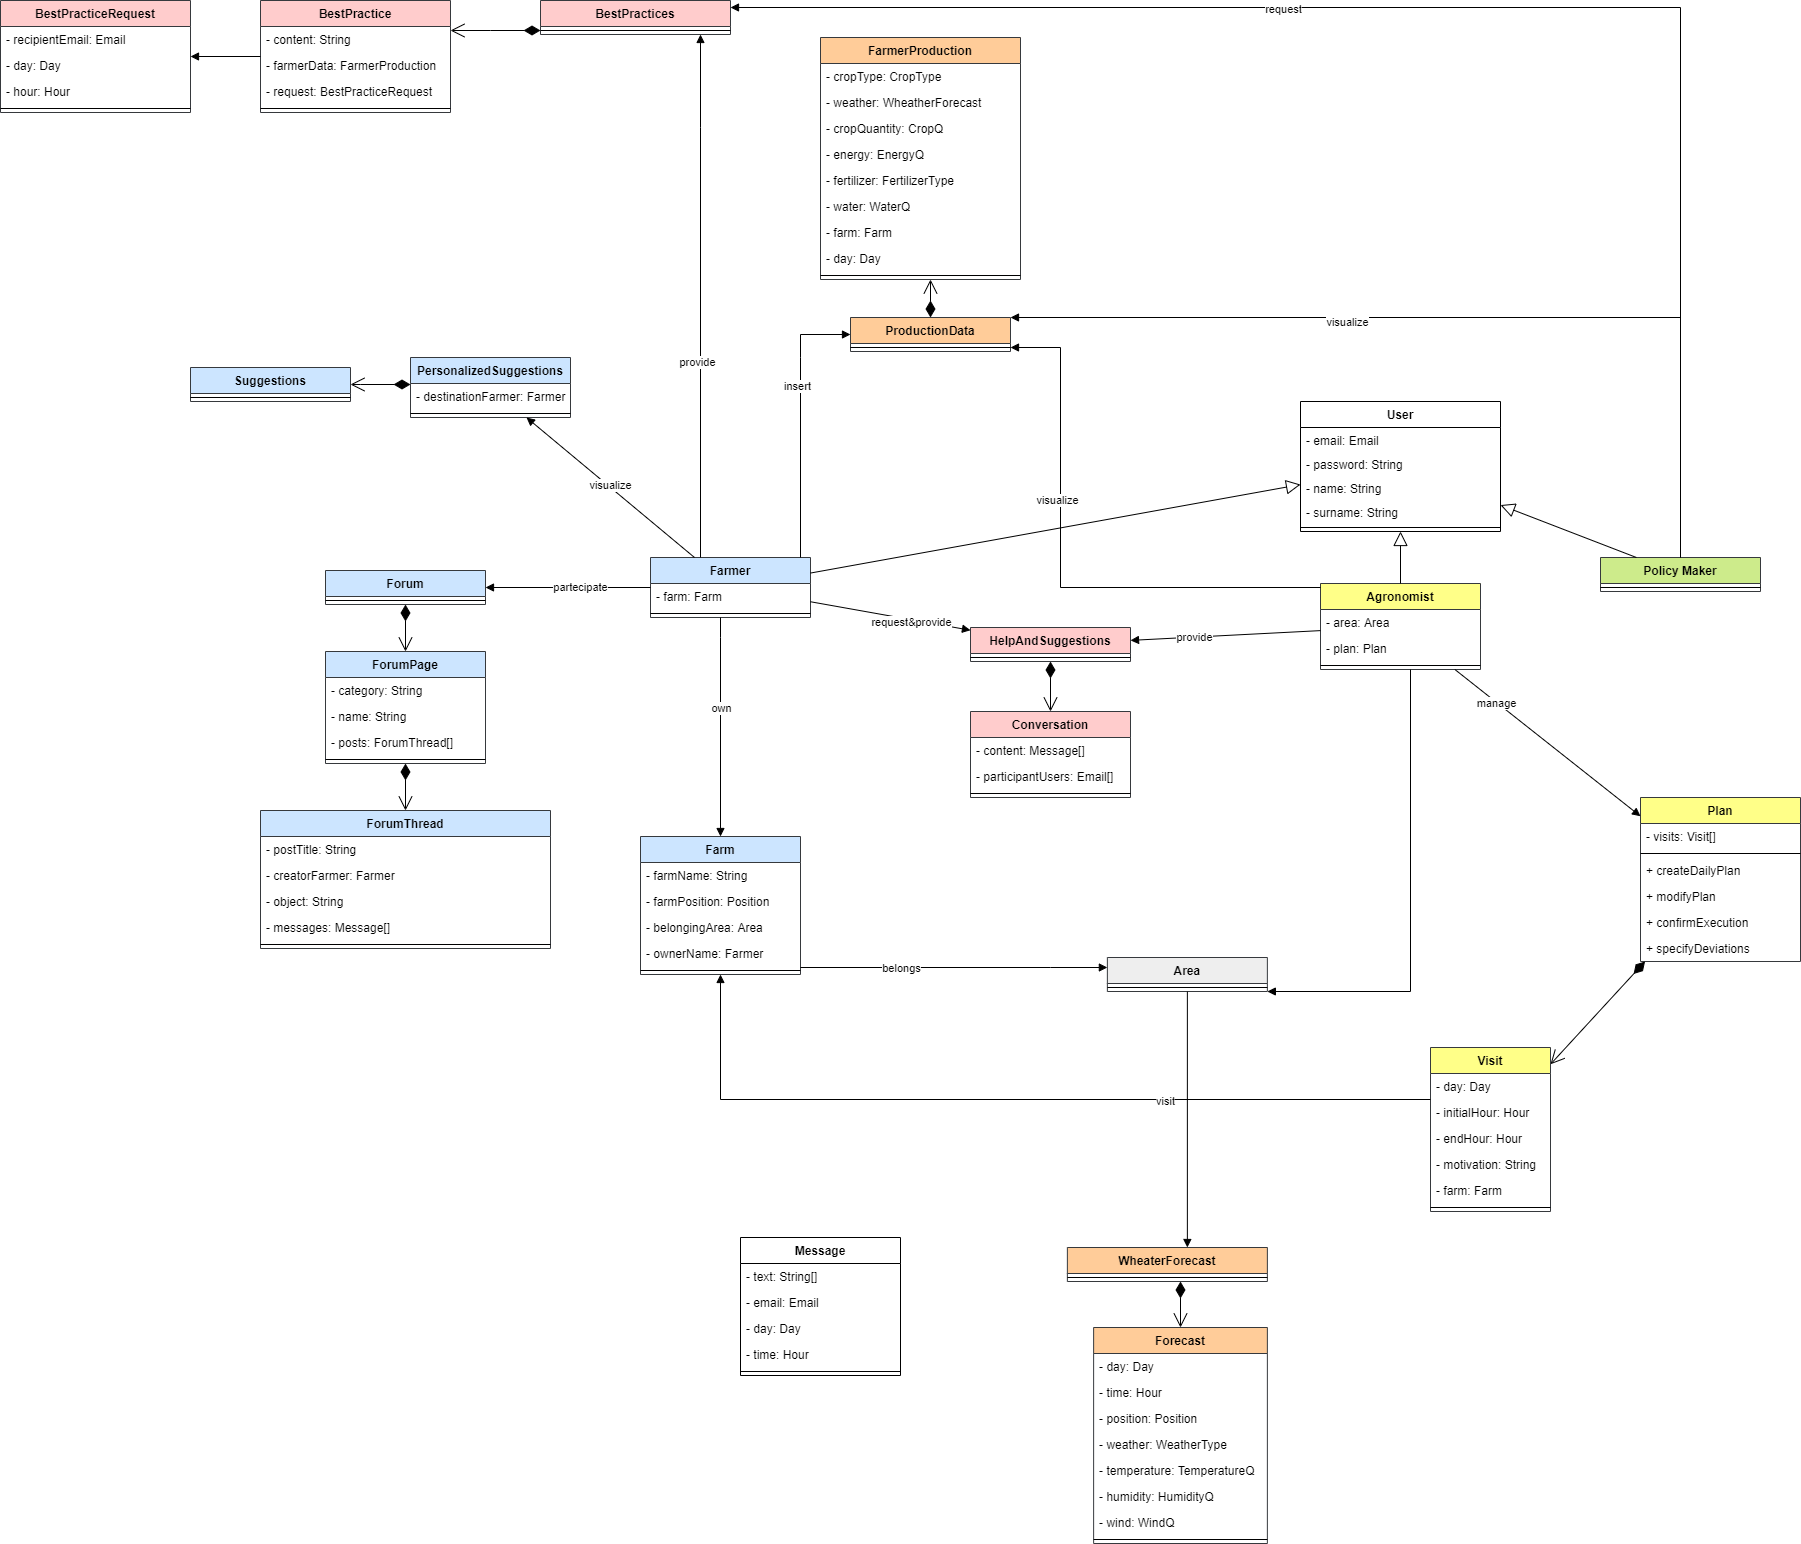
\includegraphics[width=1\textwidth]{images/ClassDiagram.png}
        \caption{\label{fig:frog}Class Diagram.}
    \end{figure}
    
    \begin{figure} [h]
        \centering
        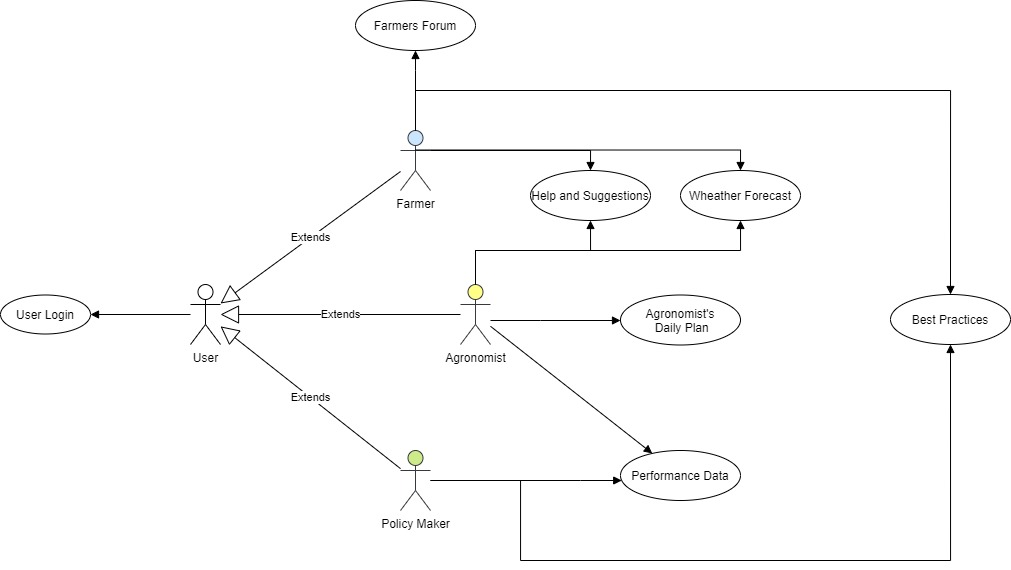
\includegraphics[width=1\textwidth]{images/UseCaseDiagram.jpg}
        \caption{\label{fig:frog}Use-Case Diagram.}
    \end{figure}

\newpage

\subsection{Product Functions}
\setlength{\parindent}{0ex}

    \begin{itemize}
        \item General user can:
            \begin{itemize}
                \item Login
                \item SignUp
            \end{itemize}
        \item Farmers can:
            \begin{itemize}
                \item Visualize relevant data
                \item Insert data about production and problems in the system
                \item Request for help and suggestions
                \item Participate in a discussion forum
            \end{itemize} 
        \item Agronomists can:
            \begin{itemize}
                \item Receive and answer to farmers requests for help
                \item Visualize and update the daily plan
                \item Confirm the execution of the daily plan
                \item Specify the deviations from the daily plan
            \end{itemize} 
        \item Policy makers can:
            \begin{itemize}
                \item See information about crops and farmers
                \item Select well performing farmers and ask them best practice
                \item Select bad performing farmers and send them suggestions
            \end{itemize}    
    \end{itemize}

\newpage

\subsection{User characteristics}

\subsubsection{Farmer}
    It’s a person engaged in agriculture, who is responsible for planting, cultivating, and managing plantations. In its work, it must take into account weather forecasts and personalized suggestions received by other farmers in order to make its production perform at its best. In addition to this, it should ask for suggestions if it has a problem, and help other farmers to resolve their own problems.

\subsubsection{Agronomists}
    It’s a person responsible for monitoring and visiting the farmers under his area of responsibility. Its job is to plan the visits to the farmers, by taking into account that every farmer must be visited at least twice a year. 
    The primary role of agronomists are in research for the benefit of farms and food; they can provide technical advice for farmers such as in making crop calendars, prescribing fertilizers to avoid misuse, in order to optimize farm production.

\subsubsection{Policy Makers}
    It’s a person responsible for identifying those farmers who are performing well to take their best practices, and those farmers who are performing badly to help them. Its aim is to monitor the results of the work of the agronomists, in order to understand if the steering initiatives are producing good results. 


\subsection{Assumptions, dependencies and constraints}

\subsubsection{Assumptions}

    \begin{itemize}
        \item D1: Users (farmers, agronomists, and policy makers) do not insert false information in the system.
        \item D2: Farmers reply as best as they can, giving the best advice, to requests for help and suggestions by other farmers (without providing unthruts).
        \item D3: Agronomists know the area they are responsible for.
        \item D4: Each area has at least one responsible agronomist.
        \item D5: Each farm is assigned to a specific area and has a unique identifier. 
        \item D6: Users have access to a stable Internet connection (e.g. to visualize weather forecasts, to participate in a discussion, to send and receive help and suggestions).
        \item D7: The location of a farm is known by the application, and the responsible agronomist is able to reach the farm.
    \end{itemize}

\subsubsection{Hardware Constraints}
The system has to run under the following worst-case conditions:

    \begin{itemize}
        \item App:
            \begin{itemize}
                \item 3G connection, at 2 Mb/s
                \item 100 MB of free space
                \item 1 GB of RAM
            \end{itemize}
        \item Web Application:
            \begin{itemize}
                \item 2 Mb/s Internet connection
                \item 800x600 resolution
            \end{itemize}
    \end{itemize}


\newpage










\section{Specific Requirements}

\subsection{Interface Requirements}

\subsubsection{User Interfaces (Farmer, Agronomist, Policy Maker)}
    
    In the figure we can see the login web page on the left and the login app screen on the right of the DREAM system. It is asked to the user to login or to create an account, and in case the user decides to register, different information can be added depending on the stakeholder it is registering. \par Firstly the user will be asked to select from 3 types of account (policy maker, farmer, agronomist) and depending on the selection different information will be required (ex. the responsible area will be asked only for the creation of an agronomist’s account). The system will then check the veracity of the inserted data and confirm the registration.
    
    \begin{figure} [h]
        \centering
        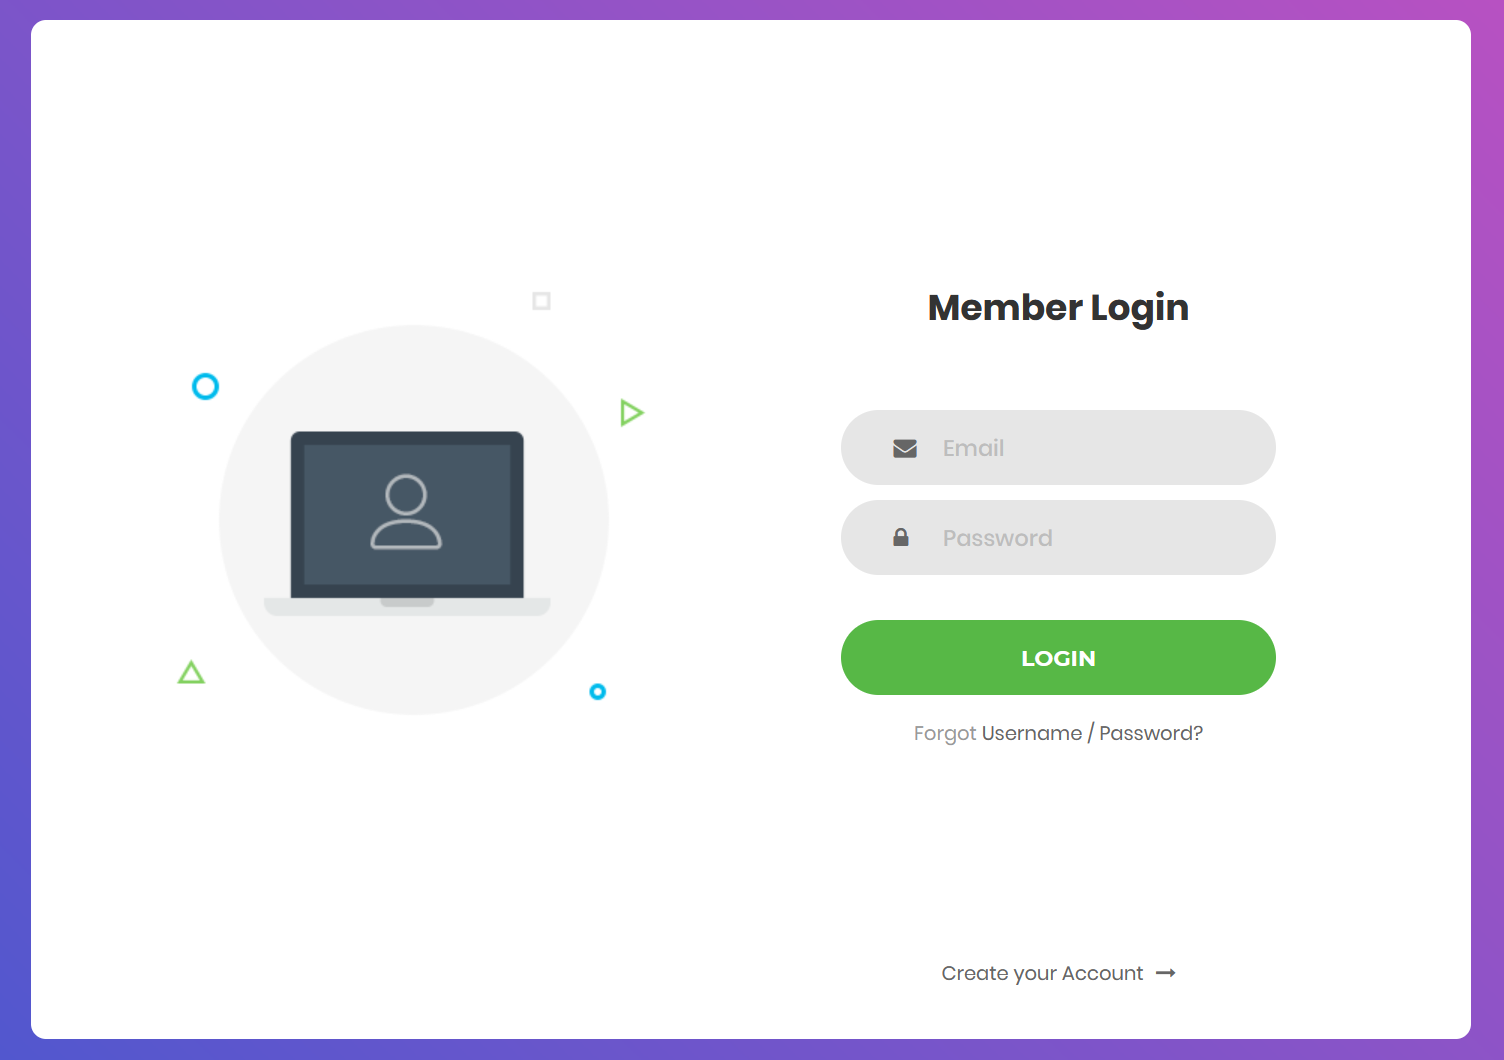
\includegraphics[width=0.5\textwidth]{images/interfaces/UserLoginWeb.png}
        \quad
        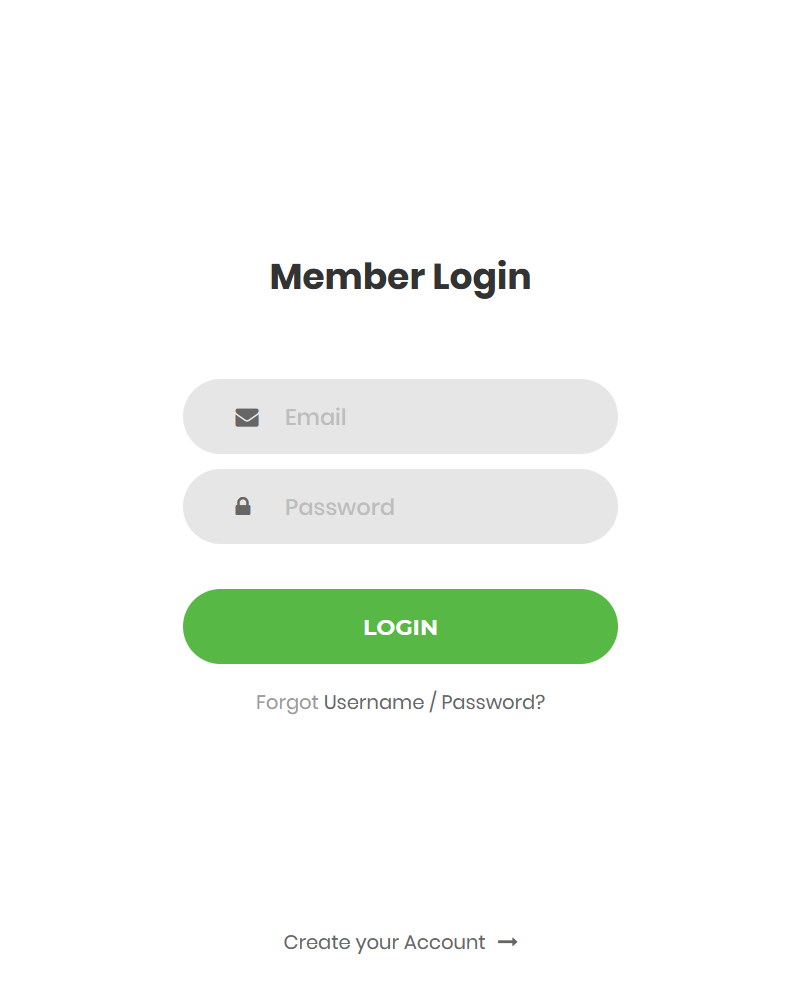
\includegraphics[width=0.4\textwidth]{images/interfaces/UserLoginApp.png}
        \quad
        \caption{\label{fig:frog}User Login.}
    \end{figure}
    
    \newpage
    
    
    

    \begin{itemize}
        \item \textbf{Farmer interface}
    \end{itemize}
    
    Farmer interface is described in figures below (web and app view). The farmer can easily access all his functionalities in the menu (at the top of the page on the web, in the retractable menu in the app), but has also some relevant information on the home page. Here it is possible to read the weather forecast of the current day and have a quick lookup on some personalized suggestions (farmer can continue reading the shown suggestion or click on “Personalized suggestion” to go to all his suggestions).
    
    \begin{figure} [h]
        \centering
        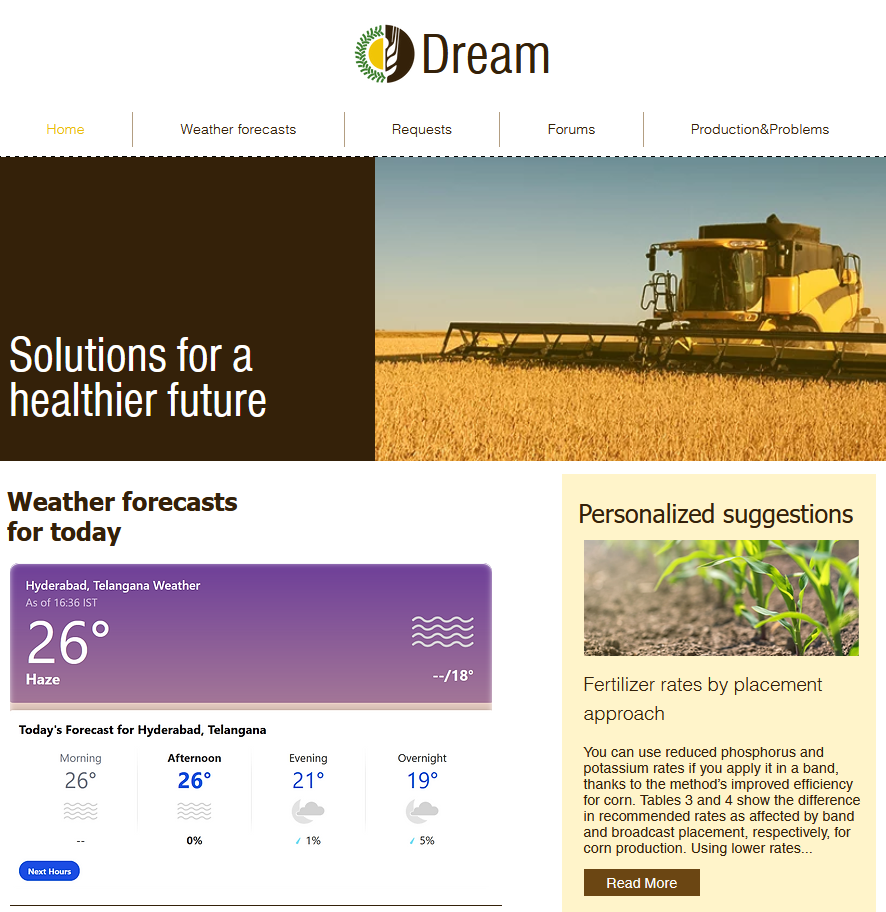
\includegraphics[width=0.7\textwidth]{images/interfaces/FarmerWeb.png}
        \quad
        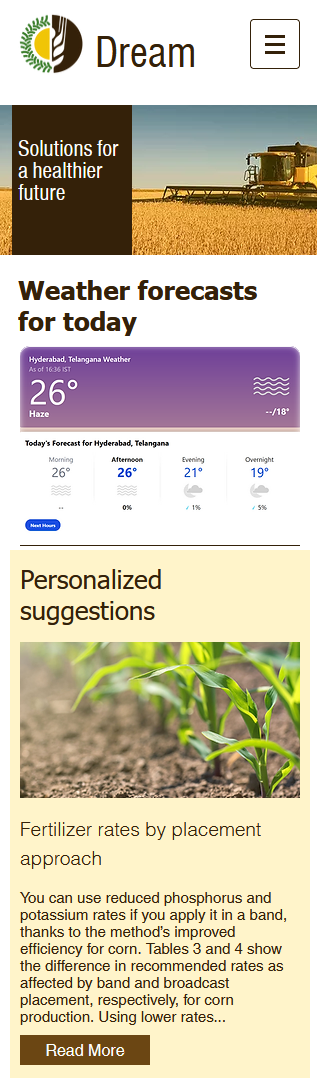
\includegraphics[width=0.2\textwidth]{images/interfaces/FarmerApp.png}
        \quad
        \caption{\label{fig:frog}Farmer Home Page.}
    \end{figure}
    
    \newpage



    \begin{itemize}
        \item \textbf{Agronomist interface}
    \end{itemize}
    
    Agronomist interface is described in figures below (web and app view). As the farmer, the agronomist can easily access all his functionalities in the menu (at the top of the page on the web, in the retractable menu in the app), but has also some relevant information on the home page. Here it is possible to read the weather forecast of the current day and have a quick lookup of today's plan.
    
    \begin{figure} [h]
        \centering
        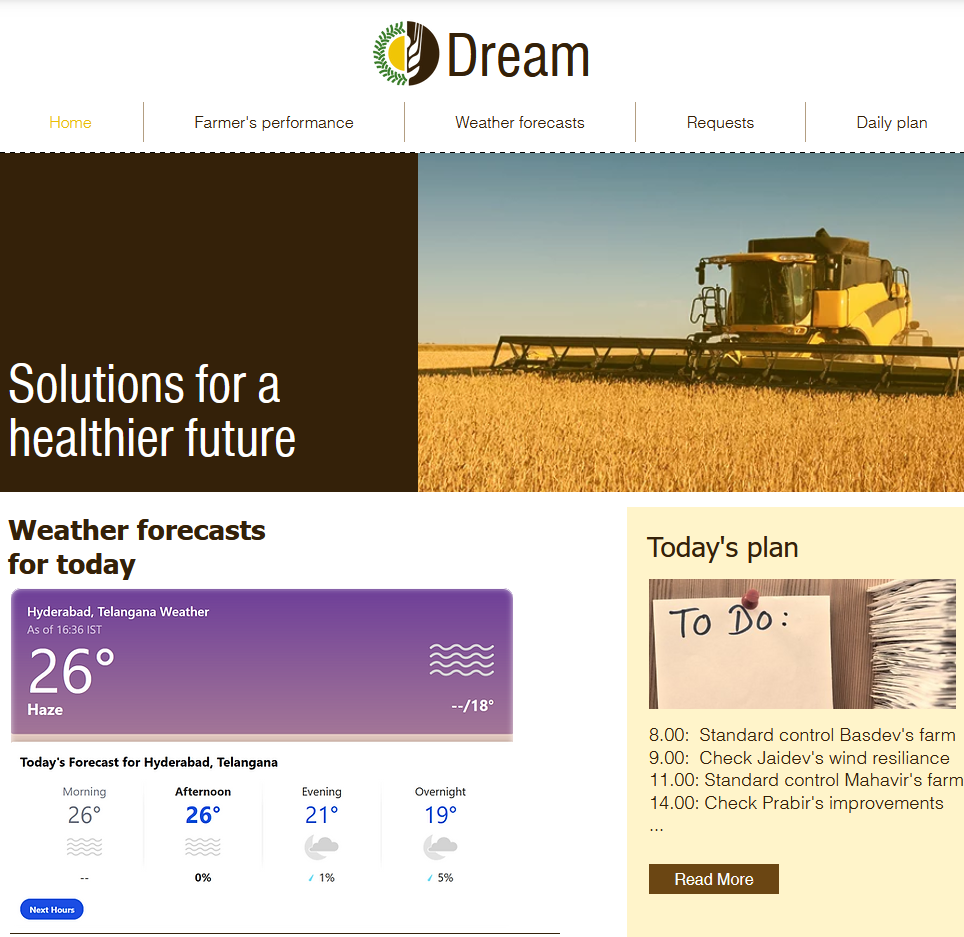
\includegraphics[width=0.7\textwidth]{images/interfaces/AgronomistWeb.png}
        \quad
        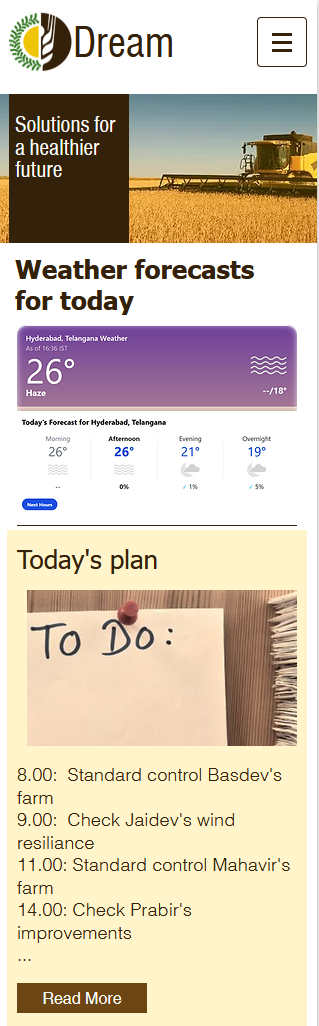
\includegraphics[width=0.2\textwidth]{images/interfaces/AgronomistApp.png}
        \quad
        \caption{\label{fig:frog}Agronomist Home Page.}
    \end{figure}
    
    \newpage
    
    
    
    \begin{itemize}
        \item \textbf{Policy Maker interface}
    \end{itemize}
    
    Agronomist interface is described in figures below (web and app view). As the farmer, the agronomist can easily access all his functionalities in the menu (at the top of the page on the web, in the retractable menu in the app), but has also some relevant information on the home page. Here it is possible to read the weather forecast of the current day and have a quick lookup of today's plan.
    
    \begin{figure} [h]
        \centering
        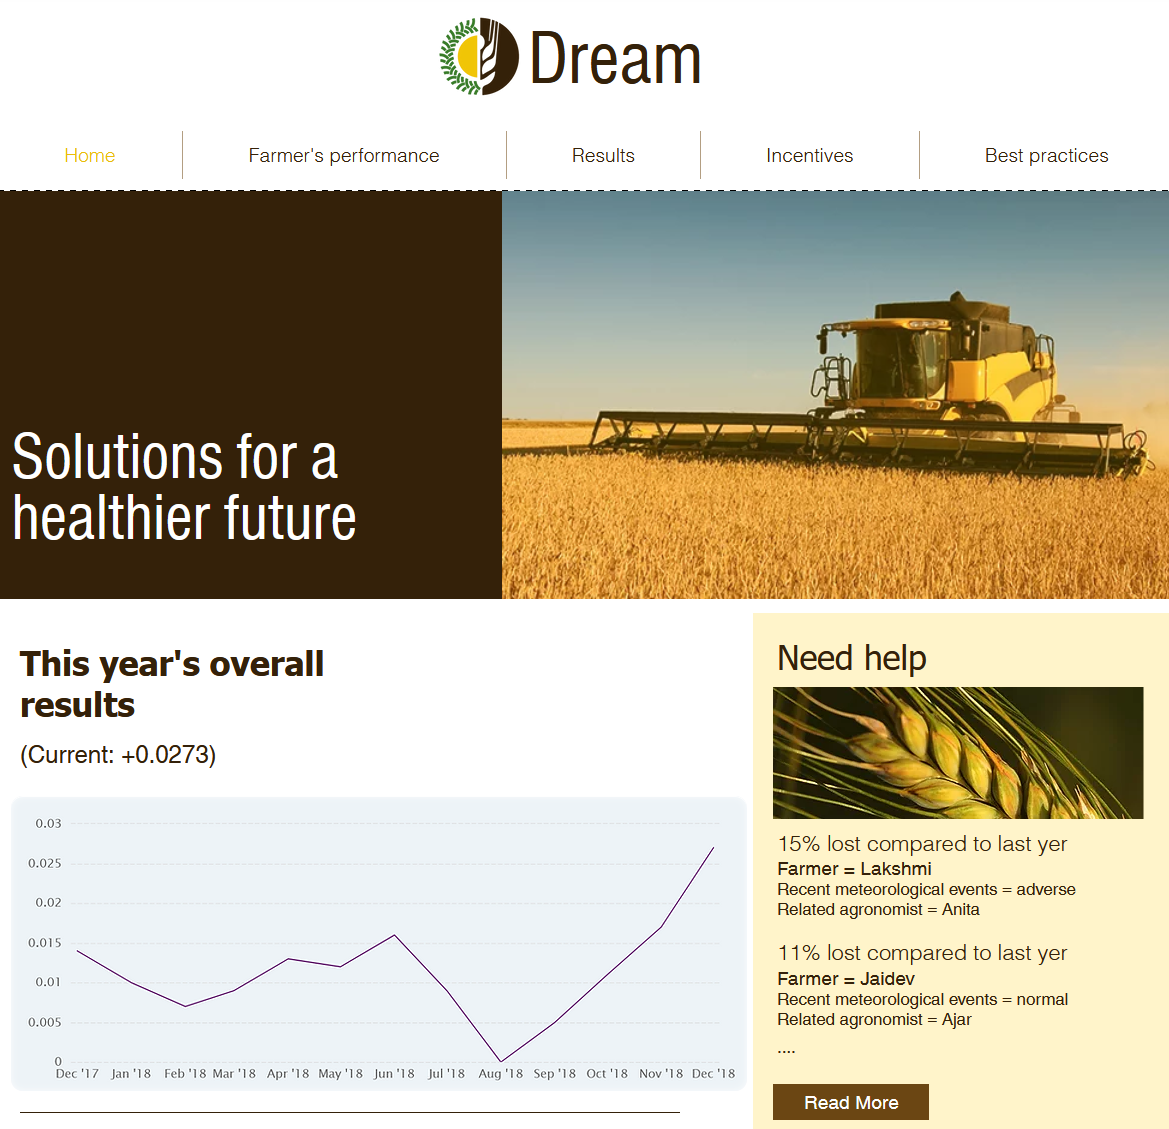
\includegraphics[width=0.7\textwidth]{images/interfaces/PolicyMakerWeb.png}
        \quad
        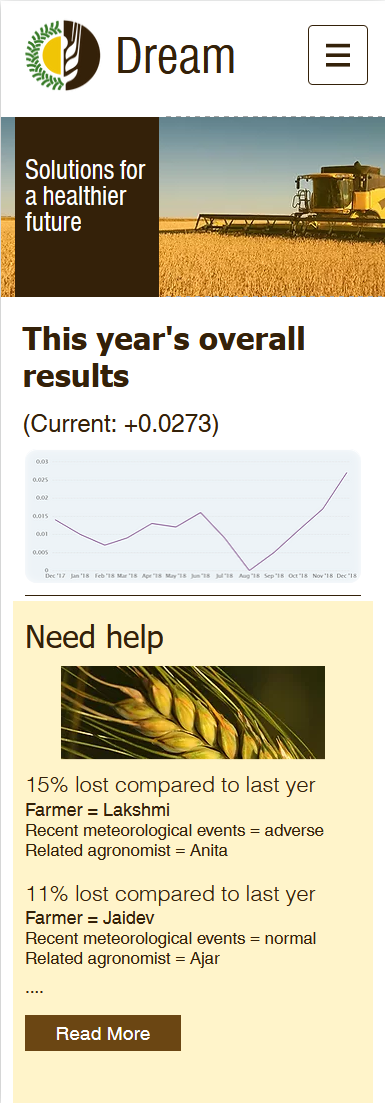
\includegraphics[width=0.2\textwidth]{images/interfaces/PolicyMakerApp.png}
        \quad
        \caption{\label{fig:frog}Policy Maker Home Page.}
    \end{figure}
    
    \newpage

\subsubsection{Hardware Interfaces}
Dream application does not provide any hardware interface. However it is possible to connect to a government database in order to automatically check the veracity of the registration data of each user.

\subsubsection{Software Interfaces}
Dream requires Java to be installed on the system, more specifically at least Java version 8 (to include functional programming). Dream can also be connected with a MySQL, SQLite or PostgreSQL government database as presented in 3.1.2.

\subsubsection{Communication Interfaces}
The clients communicate with the server via HTTPS requests.


\newpage





\subsection{Functional Requirements}

\subsubsection{Farmer Use Cases}

\begin{center}
    

    
    %FARMER SIGN UP
    
    \begin{longtable}{|c| p{10cm}|}
        \hline
            ID & 1 \\
        \hline
            Name & Farmer Sign Up \\
        \hline
            Actor & Farmer \\
        \hline
            Entry Conditions & Farmer has downloaded and opened the application on his smartphone (on the “Initial App Screen”), or has opened the web page on his personal computer (on the “Initial Web Page”). \\
        \hline
            Input & 
                    \begin{itemize}
                        \item Email to use for the registration
                        \item Personal data (name, surname)
                        \item Farm data
                    \end{itemize}\\
        \hline
            Events Flow & 
                    \begin{itemize}
                        \item Farmer clicks on “Create your Account”
                        \item System displays a list of alternatives: 
                            \begin{itemize}
                                \item Farmer
                                \item Agronomist
                                \item Policy Maker
                            \end{itemize} 
                        \item Farmer selects “Farmer”
                        \item System displays a list of fields that the farmer must     compile: 
                            \begin{itemize}
                                \item Name
                                \item Surname
                                \item Email
                                \item Password
                                \item Farm’s name
                                \item Farm’s location
                            \end{itemize}
                        \item Farmer inserts the mandatory data and accepts the Terms of Services
                        \item Farmer clicks on “Confirm” button
                        \item System displays the acceptance of registration and invites farmer to go on his inbox in order to confirm the registration
                        \item Farmer opens his inbox, checks the emails and clicks on confirmation link
                    \end{itemize}\\
        \hline
        Exit Conditions & 
                    \begin{itemize}
                        \item Farmer registration has been successful: farmer’s data are stored in the database of the system. 
                        \item Farmer can now login with his credentials (email and password)
                    \end{itemize}\\
        \hline
            Output & 
                    \begin{itemize}
                        \item The email of the farmer is stored in the database of the application
                        \item The farmer receives the email of confirmation
                    \end{itemize}\\
        \hline
            Exceptions & 
                    \begin{itemize}
                        \item Farmer inserts an email which is already stored in the database. So, after the farmer inserts his data and clicks on confirm, the application displays an error page which tells that farmer is already registered to the service and invites him to login with that email.
                        \item Farmer inserts an invalid email. So, after the farmer clicks on the confirm button, the application displays the same page and an error message, which suggests to the farmer to check the email inserted or to change it.
                        \item Farmer inserts invalid data (e.g., farmer is not the owner of the specified farm, invalid farm’s data), so, after the farmer clicks on confirm, the application displays an error page which tells that farmer has inserted invalid data and invites him to try again the registration.
                    \end{itemize}\\
        \hline
    \end{longtable}
    
    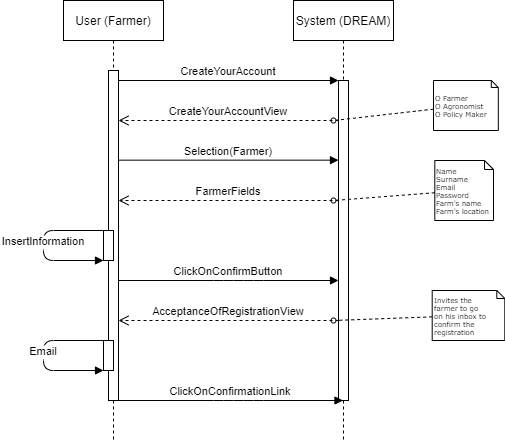
\includegraphics[width=0.8\textwidth]{images/sequenceDiagrams/1. SignUpFarmer.png} 
    \par
    \caption{\label{fig:frog}Sign Up Farmer}
        
    \newpage
    
    
    
    
    
    %FARMER VISUALIZE WHEATER FORECASTS
    
    \begin{longtable}{|c| p{10cm}|}
        \hline
            ID & 2 \\
        \hline
            Name & Farmer visualize “Weather Forecasts” \\
        \hline
            Actor & Farmer \\
        \hline
            Entry Conditions & 
                    \begin{itemize}
                        \item Farmer has logged in
                        \item Farmer is on his home page
                    \end{itemize}\\
        \hline
            Input & \\
        \hline
            Events Flow & 
                    \begin{itemize}
                        \item Farmer clicks on “Weather Forecasts”
                        \item System displays a page with the weather forecasts for the following seven days. For each day it shows four forecasts (morning, afternoon, evening, night). 
                        \item Farmer selects a day
                        \item System displays the forecasts hour by hour of the selected day (wind, max and min temperature, sunrise time, ...).
                    \end{itemize}\\
        \hline
        Exit Conditions & System successfully displays the weather forecasts for the                     day selected by the farmer\\
        \hline
            Output & Farmer sees the weather forecasts for the desired day \\
        \hline
            Exceptions & Weather forecasts are unavailable due to a problem with the              IT provider. System shows a page saying that weather forecasts             are temporarily unavailable and to try again after a while.               Then it shows the farmer's home page.\\
        \hline
    \end{longtable}
    
    
    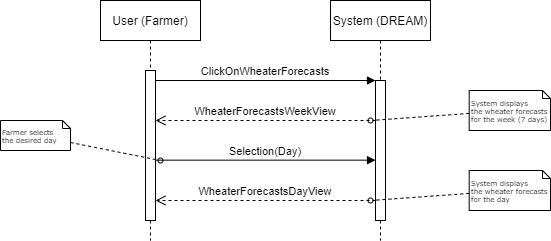
\includegraphics[width=1\textwidth]{images/sequenceDiagrams/2. FarmerWheatherForecasts.png}
    \par
    \caption{\label{fig:frog}Farmer visualizes wheater forecast}
    
    \newpage
    
    
    
    %FARMER VISUALIZE PERSONALIZED SUGGESTIONS
    
    \begin{longtable}{|c| p{10cm}|}
        \hline
            ID & 3 \\
        \hline
            Name & Farmer visualize “Personalized Suggestions” \\
        \hline
            Actor & Farmer \\
        \hline
            Entry Conditions & 
                                \begin{itemize}
                                    \item Farmer has logged in
                                    \item Farmer is on his home page
                                \end{itemize}\\
        \hline
            Input & \\
        \hline
            Events Flow & 
                    \begin{itemize}
                        \item Farmer clicks on “Personalized Suggestions” 
                            \begin{itemize}
                                \item If farmer clicks on “Read More” on the preview of a suggestion on the Home Page jump directly to last point
                            \end{itemize} 
                        \item -	System displays a page with the preview of all his suggestions (which fertilizer to use, which crops to plant) 
                        \item Farmer selects a suggestion
                        \item System displays the selected suggestion
                    \end{itemize}\\
        \hline
        Exit Conditions & System successfully displays the selected suggestion\\
        \hline
            Output & Farmer sees the selected suggestion\\
        \hline
            Exceptions & Chosen personalized suggestion has been removed while the farmer was reading its preview. When it is selected the system shows a message saying the suggestion is no more pertinent to him and displays its home page.\\
        \hline
    \end{longtable}
   
    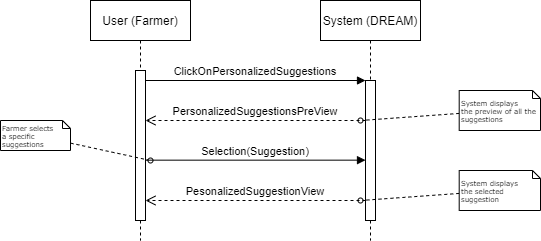
\includegraphics[width=1\textwidth]{images/sequenceDiagrams/3. FarmerPersonalizedSuggestions.png}
    \par
    \caption{\label{fig:frog}Farmer visualize “Personalized Suggestions”}

    \newpage
    
    
    %FARMER INSERT PRODUCTION DATA
    
    \begin{longtable}{|c| p{10cm}|}
        \hline
            ID & 4 \\
        \hline
            Name & Farmer insert “Production Data” \\
        \hline
            Actor & Farmer \\
        \hline
            Entry Conditions & 
                                \begin{itemize}
                                    \item Farmer has logged in
                                    \item Farmer is on his home page
                                \end{itemize}\\
        \hline
            Input & \begin{itemize}
                        \item Amount of corn produces
                        \item Amount of energy used per unit
                        \item Amount of fertilizer used per unit
                        \item Amount of water used per unit
                    \end{itemize} \\
        \hline
            Events Flow &   \begin{itemize}
                                \item Farmer clicks on “ProductionAndProblems” 
                                \item System asks if the farmer wants to access “Production Data” or wants to “Report a Problem”
                                \item Farmer selects “Production Data”
                                \item System displays a page with farmer’s production data’s history and the button “Insert Data”
                                \item Farmer selects the button (if selects an already present production data the system automatically opens the page of “Insert Data” with old datas copied in it, and if saved the old production will be automatically deleted)
                                \item System displays the page “Insert Production Data”
                                \item Farmer inserts the amount of corn produced and the amount of energy, water and fertilizer used per unit.
                                \item Farmer clicks “Save” button
                                \item System shows the message “Production has been inserted successfully” 
                                \item System displays farmer’s home page
                            \end{itemize} \\
        \hline
            Exit Conditions & Production data has been successfully added to the system\\
        \hline
            Output & Farmer’s production data is stored in the database of the application\\
        \hline
            Exceptions &\\
        \hline
    \end{longtable}
    
    \newpage
    
    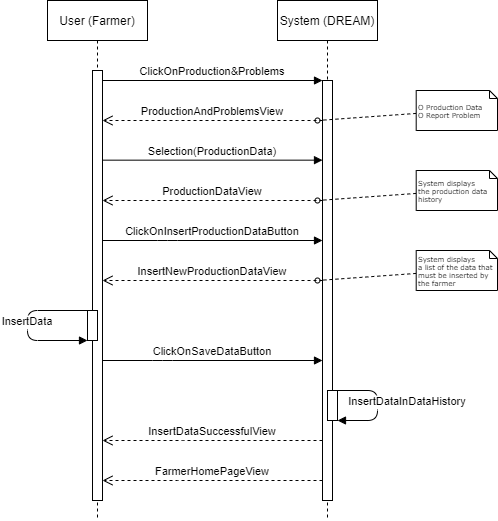
\includegraphics[width=1\textwidth]{images/sequenceDiagrams/4. FarmerInsertProductionData.png}
    \par 
    \caption{\label{fig:frog}Farmer insert “Production Data”}

    \newpage
    
    
    
    
    
    
    %FARMER REPORT A PROBLEM
    
    \begin{longtable}{|c| p{10cm}|}
        \hline
            ID & 5 \\
        \hline
            Name & Farmer “Report a Problem”  \\
        \hline
            Actor & Farmer \\
        \hline
            Entry Conditions & 
                                \begin{itemize}
                                    \item Farmer has logged in
                                    \item Farmer is on his home page
                                \end{itemize}\\
        \hline
            Input & Description of the problem \\
        \hline
            Events Flow &   \begin{itemize}
                                \item Farmer clicks on “ProductionAndProblems” 
                                \item System asks if the farmer wants to access “Production Data” or wants to “Report a Problem”
                                \item Farmer selects “Report a Problem”
                                \item System displays a page where it asks a brief description of the problem and shows the agronomists responsible of the farmer’s area
                                \item Farmer inserts the description of the problem and selects an agronomist
                                \item Farmer selects “Report” button
                                \item System sends a notification of “Bad Performing Farmer” to the selected agronomist
                                \item System shows the message “Problem has been reported successfully” 
                                \item System displays farmer’s home page
                            \end{itemize} \\
        \hline
            Exit Conditions & Problem report has been successfully added to the system and the agronomist has been notified\\
        \hline
            Output & Problem report is stored in the database of the application and a notification has been sent to the agronomist\\
        \hline
            Exceptions & Farmer inserts a description of more than 400 words. Since it is no longer a brief description, when the farmer tries to save the report the system shows the message “Description must fit in 400 words” and the number of written words, and it remains on the same page (in order to let the user shorten the text) \\
        \hline
    \end{longtable}
    
    \newpage
    
    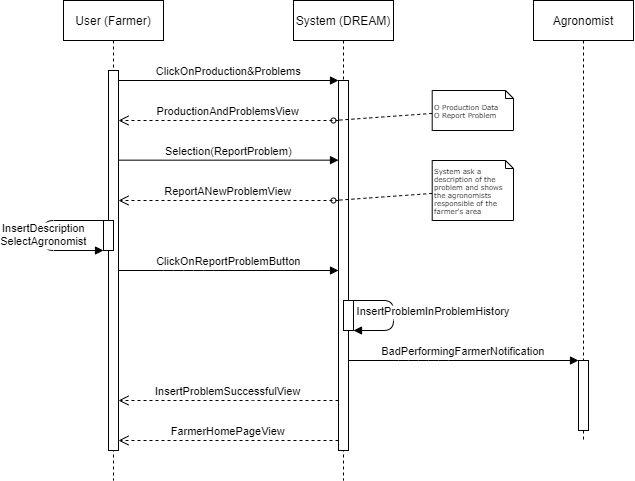
\includegraphics[width=1\textwidth]{images/sequenceDiagrams/5. FarmerReportProblem.png}
    \par
    \caption{\label{fig:frog}Farmer “Report a Problem”}

    \newpage
    
    

    %FARMER REQUESTS FOR HELP AND SUGGESTIONS
    
    \begin{longtable}{|c| p{10cm}|}
        \hline
            ID & 6 \\
        \hline
            Name & Farmer requests for “Help and Suggestions”  \\
        \hline
            Actor & Farmer \\
        \hline
            Entry Conditions & 
                                \begin{itemize}
                                    \item Farmer has logged in
                                    \item Farmer is on his home page
                                \end{itemize}\\
        \hline
            Input & \begin{itemize}
                        \item Description of the request
                        \item Optional: Identifier of the addressee (specific agronomist/farmer)
                    \end{itemize} \\
        \hline
            Events Flow &   \begin{itemize}
                                \item Farmer clicks on “Requests”
                                \item System displays a page with a list of the most recent received requests and a button “Create New Request”
                                \item Farmer selects the button “Create New Request”
                                \item System displays a page with text field (to store the request) and a list of possible addressee (receiver of the request): 
                                        \begin{itemize}
                                            \item Specific Agronomist
                                            \item Specific farmer
                                            \item All farmers of my area
                                            \item All agronomist of my area
                                        \end{itemize}

                                \item Farmer insert the description of the request
                                \item Farmer selects the receiver
                                        \begin{itemize}
                                            \item In case a specific agronomist/farmer has been selected, the system lets the farmer insert an identifier of the receiver
                                        \end{itemize}
                                \item Farmer selects “Send” button
                                \item System sends a notification to receiver/s
                                \item System shows a message saying “Message sent” 
                                \item System displays farmer’s home page
                            \end{itemize} \\
        \hline
            Exit Conditions & Request has been sent successfully\\
        \hline
            Output &    \begin{itemize}
                            \item The request is stored in the database of the application
                            \item Receivers gets a notification
                        \end{itemize}\\
        \hline
            Exceptions &    \begin{itemize}
                                \item Farmer inserts an invalid identifier of the receiver. The system shows the message “Invalid receiver” and displays the page of the request to let the farmer modify it.
                                \item Farmer inserts a message in the text field of over 400 characters. Systems shows an error message “A request can have at most 400 characters” and displays again the page with the text field (filled with old message) and the button.
                            \end{itemize} \\
        \hline
    \end{longtable}
    
    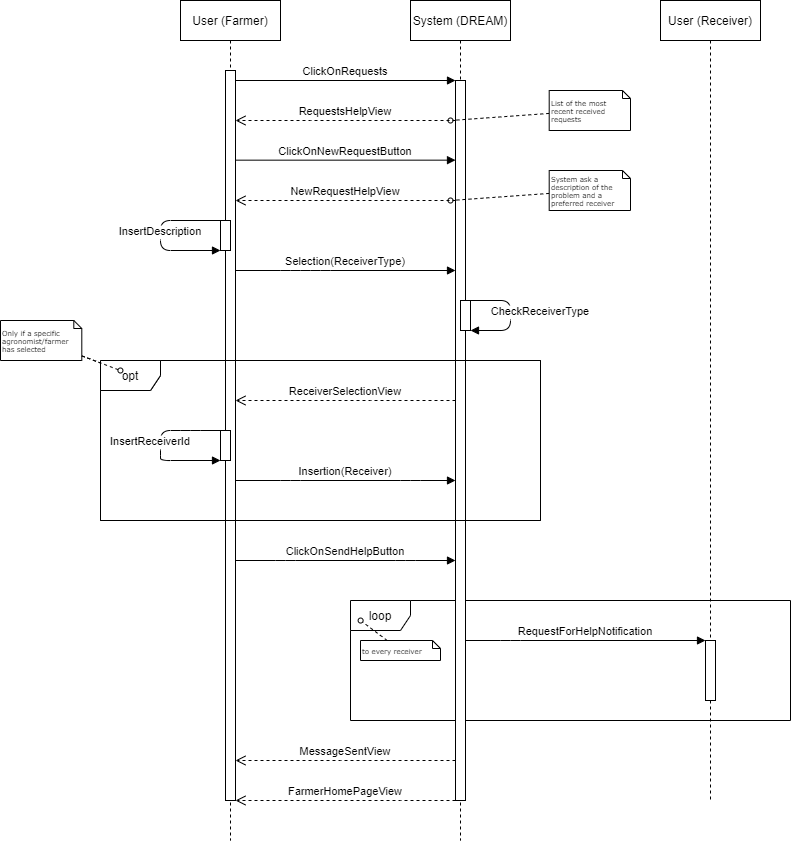
\includegraphics[width=0.9\textwidth]{images/sequenceDiagrams/6. FarmerRequestHelp.png}
    \par
    \caption{\label{fig:frog}Farmer requests for Help and Suggestions}

    \newpage


    
    
    
   
   
    %FARMER RESPONDS TO A HELP AND SUGGESTIONS
    
    \begin{longtable}{|c| p{10cm}|}
        \hline
            ID & 7 \\
        \hline
            Name & Farmer responds to a “Request for Help and Suggestions”  \\
        \hline
            Actor & Farmer \\
        \hline
            Entry Conditions & 
                                \begin{itemize}
                                    \item Farmer has logged in
                                    \item Farmer has received a request for help
                                \end{itemize}\\
        \hline
            Input & Text of the response \\
        \hline
            Events Flow &   \begin{itemize}
                                \item Farmer clicks on “Requests”
                                        \begin{itemize}
                                            \item If farmer directly clicks on the notification of the request, jump directly to 4th point
                                        \end{itemize}
                                \item System displays a page with a list of the most recent received requests and a button “Create New Request”
                                \item Farmer selects a request
                                \item System displays the request and an “Answer” button
                                \item Farmer reads the request and selects the “Answer” button
                                \item System displays a text field for the response and a “Send” button
                                \item Farmer inserts the text and clicks on the “Send” button
                                \item System shows a message saying “Message sent” 
                                \item System displays farmer’s home page
                                \item System sends a notification to sender of the request
                            \end{itemize} \\
        \hline
            Exit Conditions & Response has been sent successfully\\
        \hline
            Output &    \begin{itemize}
                            \item The response is stored in the database of the application
                            \item Receivers gets a notification
                        \end{itemize}\\
        \hline
            Exceptions &    \begin{itemize}
                                \item Farmer selects the “Send” button with an empty message for the response. Systems shows an error message ”A response can’t be empty” and displays again the page with the text field and the button.
                                \item Farmer inserts a message in the text field of over 400 characters. Systems shows an error message “A response can have at most 400 characters” and displays again the page with the text field (filled with old message) and the button.
                            \end{itemize} \\
        \hline
    \end{longtable}
    
    \newpage

    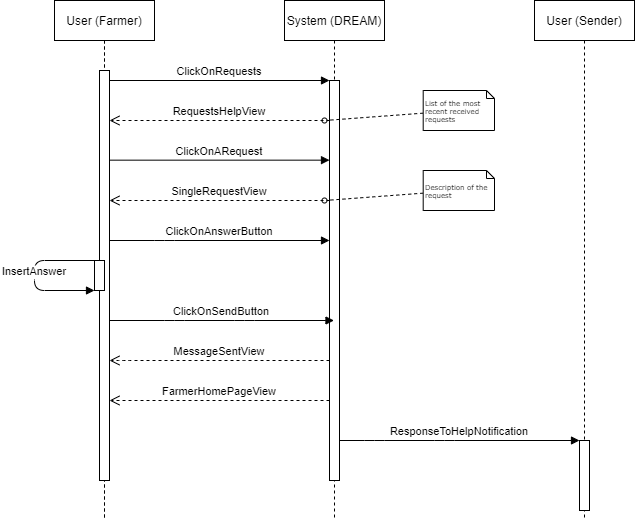
\includegraphics[width=1.0\textwidth]{images/sequenceDiagrams/7. FarmerRespondHelp.png}
    \par
    \caption{\label{fig:frog}Farmer responds to a “Request for Help and Suggestions”}
    
    \newpage






    %FARMER WRITES A NEW POST ON A DISCUSSION FORUM
    
    \begin{longtable}{|c| p{10cm}|}
        \hline
            ID & 8 \\
        \hline
            Name & Farmer writes a new post on a discussion forum\\
        \hline
            Actor & Farmer \\
        \hline
            Entry Conditions & 
                                \begin{itemize}
                                    \item Farmer has logged in
                                    \item Farmer is on his home page
                                \end{itemize}\\
        \hline
            Input & Text of the response \\
        \hline
            Events Flow &   \begin{itemize}
                                \item Farmer clicks on “Forums”
                                \item System displays a page with different topics 
                                \item Farmer selects the topic related to his message
                                \item System displays:
                                            \begin{itemize}
                                                \item The latest messages related to the selected topic
                                                \item A search bar to permit the search of messages containing the written key words
                                                \item The button “New Post” 
                                                \item The button “Subscribe” (or “Unsubscribe” if already subscribed)
                                            \end{itemize}
                                \item Farmer selects “New Post” button
                                \item System displays a text field for the post and a “Send” button
                                \item Farmer writes the message and selects the “Send” button
                                \item System shows a message saying “New Post Created”
                                \item System displays forum’s page of the same topic
                                \item System sends a notification to all the farmers subscribed to the topic of the post
                            \end{itemize} \\
        \hline
            Exit Conditions & Post has been successfully added\\
        \hline
            Output &    \begin{itemize}
                            \item The post is stored in the database of the application
                            \item Farmer subscribed to the topic of the post gets a notification
                        \end{itemize}\\
        \hline
            Exceptions &    \begin{itemize}
                                \item Farmer selects the “Send” button with an empty message for the post. Systems shows an error message “A post can’t be empty” and displays again the page with the text field and the button.
                                \item Farmer inserts a message in the text field of over 300 characters. Systems shows an error message “A post can have at most 300 characters” and displays again the page with the text field (filled with old message) and the button.
                            \end{itemize} \\
        \hline
    \end{longtable}
    
    \newpage

    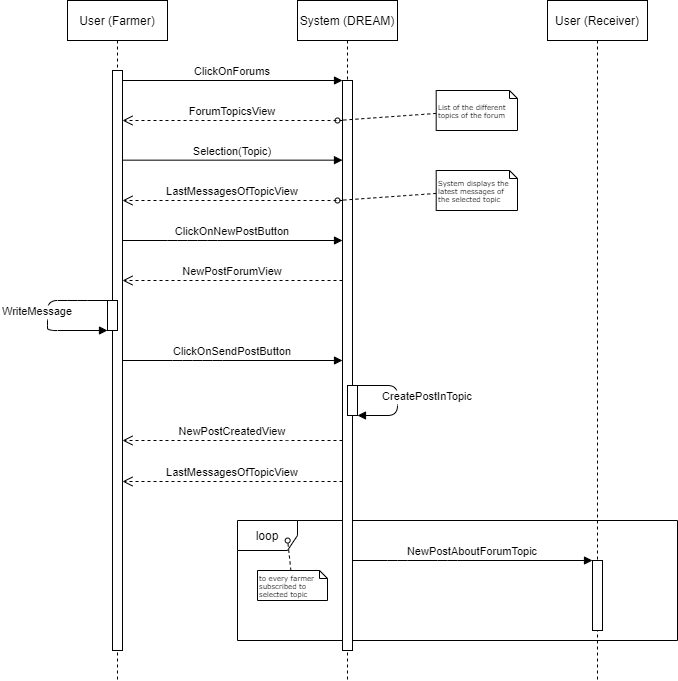
\includegraphics[width=1.0\textwidth]{images/sequenceDiagrams/8. FarmerNewPostDiscForum.png}
    \par
    \caption{\label{fig:frog}Farmer writes a new post on a discussion forum}

    \newpage
    
    
    
    
    
    
    %FARMER RESPONDS ON A DISCUSSION FORUM
    
    \begin{longtable}{|c| p{10cm}|}
        \hline
            ID & 9 \\
        \hline
            Name & Farmer responds on a discussion forum\\
        \hline
            Actor & Farmer \\
        \hline
            Entry Conditions & 
                                \begin{itemize}
                                    \item Farmer has logged in
                                    \item Farmer is on his home page
                                \end{itemize}\\
        \hline
            Input & Message to be sent \\
        \hline
            Events Flow &   \begin{itemize}
                                \item Farmer clicks on “Forums”
                                \item System displays a page with different topics  
                                \item Farmer selects the topic
                                \item System displays:
                                            \begin{itemize}
                                                \item The latest messages related to the selected topic
                                                \item A search bar to permit the search of messages containing the written key words
                                                \item The button “New Post” 
                                                \item The button “Subscribe” (or “Unsubscribe” if already subscribed)
                                            \end{itemize}
                                \item Farmer selects the search bar and types some words to identify the message. Then press enter.
                                \item System shows a page containing the messages containing the selected words
                                \item Farmer selects a message
                                \item System shows the message with the most recent responses and an “Answer” button
                                \item Farmer selects the “Answer” button
                                \item System displays a text field for the response and a “Send” button
                                \item Farmer inserts the text and presses the “Send” button
                                \item System shows a message saying “Response sent” 
                                \item System displays again the message selected before with the most recent responses and the “Answer” button
                                \item System sends a notification to all the farmers subscribed to the topic of the post (and to the creator of the post even if not subscribed to the topic)
                            \end{itemize} \\
        \hline
            Exit Conditions & Response has been sent successfully\\
        \hline
            Output &    \begin{itemize}
                            \item The response is stored in the database of the application
                            \item Receivers gets a notification
                        \end{itemize}\\
        \hline
            Exceptions &    \begin{itemize}
                                \item Farmer selects the “Send” button with an empty message for the response. Systems shows an error message ”A post can’t be empty” and displays again the page with the text field and the button.
                                \item Farmer inserts a message in the text field of over 300 characters. Systems shows an error message “A post can have at most 300 characters” and displays again the page with the text field (filled with old message) and the button.
                            \end{itemize} \\
        \hline
    \end{longtable}
    
    \newpage
    
    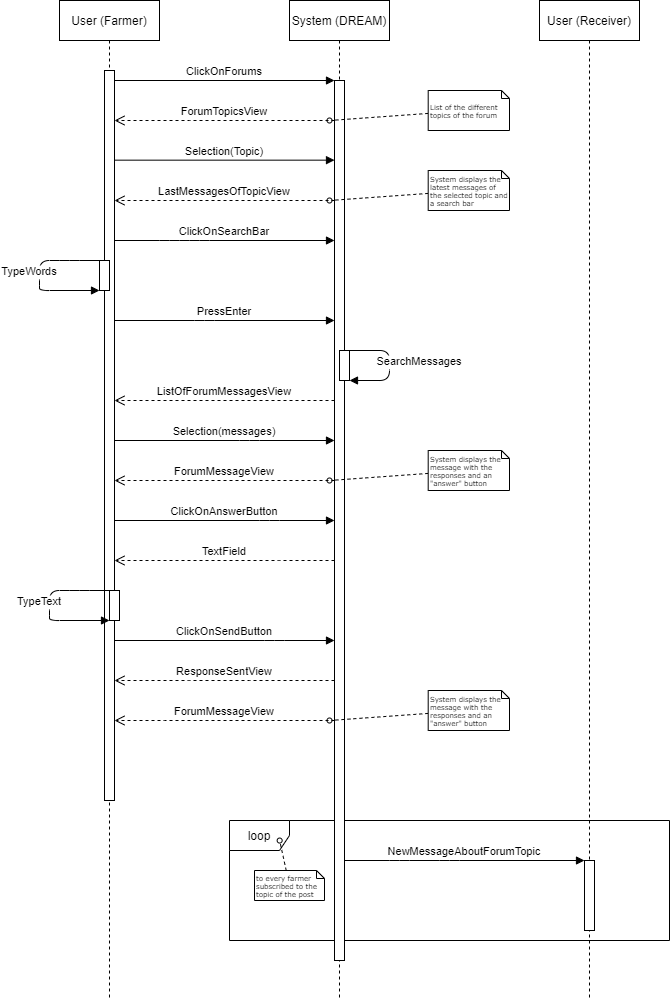
\includegraphics[width=1.0\textwidth]{images/sequenceDiagrams/9. FarmerRespondDiscForum.png} 
    \par
    \caption{\label{fig:frog}Farmer responds on a discussion forum}
    
    \newpage
    
    
    
    
    
    
    %FARMER SUBSCRIBES TO A TOPIC
    
    \begin{longtable}{|c| p{10cm}|} 
        \hline
            ID & 10 \\
        \hline
            Name & Farmer subscribes to a topic\\
        \hline
            Actor & Farmer \\
        \hline
            Entry Conditions & 
                                \begin{itemize}
                                    \item Farmer has logged in
                                    \item Farmer is on his home page
                                    \item Farmer is not already subscribed to the topic
                                \end{itemize}\\
        \hline
            Input & \\
        \hline
            Events Flow &   \begin{itemize}
                                \item Farmer clicks on “Forums”
                                \item System displays a page with different topics  
                                \item Farmer selects the topic
                                \item System displays:
                                            \begin{itemize}
                                                \item The latest messages related to the selected topic
                                                \item A search bar to permit the search of messages containing the written key words
                                                \item The button “New Post” 
                                                \item The button “Subscribe”
                                            \end{itemize}
                                \item Farmer clicks the button “Subscribe”
                                \item System shows a message saying “You have successfully subscribed to the topic, you will be notified when a new message is added to this topic section” 
                                \item System displays the page of the chosen topic
                            \end{itemize} \\
        \hline
            Exit Conditions & Subscription has been successfully performed\\
        \hline
            Output & The subscription is stored in the database of the application\\
        \hline
            Exceptions & \\
        \hline
    \end{longtable}
    
    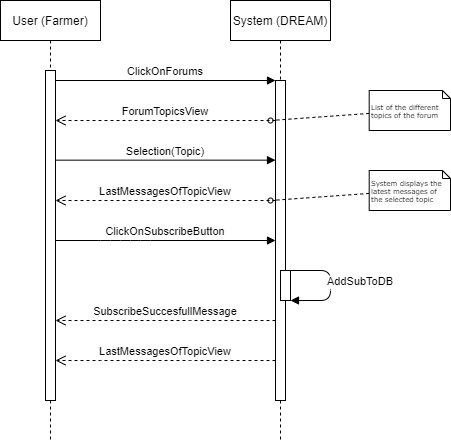
\includegraphics[width=1.0\textwidth]{images/sequenceDiagrams/10. FarmerTopicSubscribe.png}
    \par
    \caption{\label{fig:frog}Farmer subscribes to a topic}

    \newpage
    
    
    
    
    
    %FARMER UNSUBSCRIBES TO A TOPIC
    
    \begin{longtable}{|c| p{10cm}|}
        \hline
            ID & 11 \\
        \hline
            Name & Farmer unsubscribes to a topic\\
        \hline
            Actor & Farmer \\
        \hline
            Entry Conditions & 
                                \begin{itemize}
                                    \item Farmer has logged in
                                    \item Farmer is on his home page
                                    \item Farmer is  already subscribed to the topic
                                \end{itemize}\\
        \hline
            Input & \\
        \hline
            Events Flow &   \begin{itemize}
                                \item Farmer clicks on “Forums”
                                \item System displays a page with different topics  
                                \item Farmer selects the topic
                                \item System displays:
                                            \begin{itemize}
                                                \item The latest messages related to the selected topic
                                                \item A search bar to permit the search of messages containing the written key words
                                                \item The button “New Post” 
                                                \item The button “Unsubscribe”
                                            \end{itemize}
                                \item Farmer clicks the button “Unsubscribe”
                                \item System shows a message saying “You have successfully unsubscribed to the topic, you will no more be notified when a new message is added to this topic section” 
                                \item Farmer displays farmer’s home page
                            \end{itemize} \\
        \hline
            Exit Conditions & Unsubscription has been successfully performed \\
        \hline
            Output & The subscription is removed from the database of the application\\
        \hline
            Exceptions & \\
        \hline
    \end{longtable}
    
    \newpage
    
    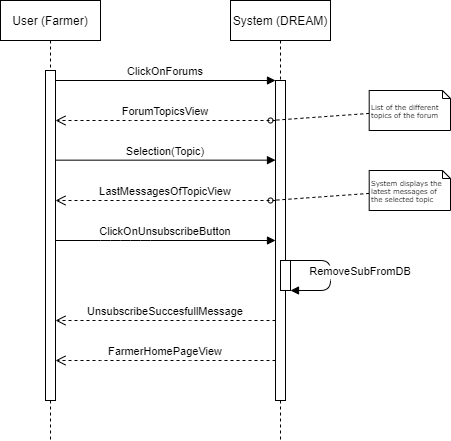
\includegraphics[width=1.0\textwidth]{images/sequenceDiagrams/11. FarmerTopicUnsubscribe.png}
    \par
    \caption{\label{fig:frog}Farmer unsubscribes from a topic}

    \newpage
    
    
    
    
    
    %FARMER INSERTS BEST PRACTICES
    
    \begin{longtable}{|c| p{10cm}|}
        \hline
            ID & 12 \\
        \hline
            Name & Farmer inserts “Best Practices”\\
        \hline
            Actor & Farmer \\
        \hline
            Entry Conditions & 
                                \begin{itemize}
                                    \item Farmer has logged in
                                    \item Farmer has received a notification “Request for best practices”
                                \end{itemize}\\
        \hline
            Input & Best practices\\
        \hline
            Events Flow &   \begin{itemize}
                                \item Farmer clicks on the notification “Request for Best Practices”
                                \item System displays a page with the text of the received request, a text field for the response and a button “Send” 
                                \item Farmer inserts the response and clicks “Send” button
                                \item System shows a message “Best practices successfully sent”
                                        \begin{itemize}
                                            \item The system doesn’t actually send the best practices to the policy maker but instead collects some info useful to identify the condition of the farmer (location, production, recent weather...) and stores the response associated with that information in the database. These best practices will be shown as personalized suggestions to Farmers in a similar condition.
                                        \end{itemize}
                            \end{itemize} \\
        \hline
            Exit Conditions & Best practices have successfully been inserted \\
        \hline
            Output & Best practices and farmer’s condition are stored in the database of the application\\
        \hline
            Exceptions & \begin{itemize}
                            \item Farmer selects the “Send” button with an empty message inserted. Systems shows an error message ”You can’t respond with an empty text” and displays again the page with the text field and the button.
                            \item Farmer inserts a message in the text field of over 200 characters. Systems shows an error message “A best practice can have at most 200 characters” and displays again the page with the text field (filled with old message) and the button.
                        \end{itemize}\\
        \hline
    \end{longtable}
    
    \newpage
    
    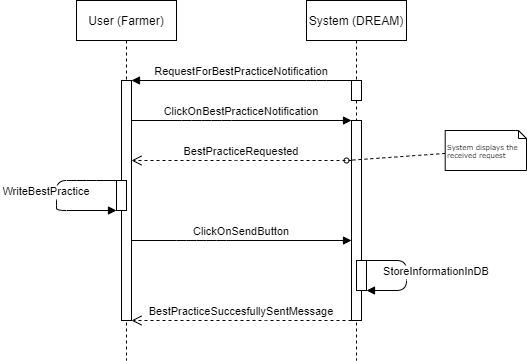
\includegraphics[width=1.0\textwidth]{images/sequenceDiagrams/12. FarmerInsertBestPractice.png}
    \par
    \caption{\label{fig:frog}Farmer inserts “Best Practices”}

    \newpage
    
\end{center} 



\subsubsection{Agronomists use cases}

\begin{center}

    
    %AGRONOMIST SIGN UP
    
    \begin{longtable}{|c| p{10cm}|}
        \hline
            ID & 13 \\
        \hline
            Name & Sign Up Agronomist\\
        \hline
            Actor & Agronomist \\
        \hline
            Entry Conditions & Agronomist has downloaded and opened the application on his smartphone (on the “Initial App Screen”), or has opened the web page on his personal computer (on the “Initial Web Page”).\\
        \hline
            Input & \begin{itemize}
                        \item Email to use for the registration
                        \item Personal data (name, surname)
                        \item Responsible area data
                    \end{itemize}\\
        \hline
            Events Flow &   \begin{itemize}
                                \item Agronomist clicks on “Create your Account”
                                \item System displays a list of alternatives:
                                        \begin{itemize}
                                            \item Farmer
                                            \item Agronomist
                                            \item Policy Maker
                                        \end{itemize}
                                \item Agronomist selects “Agronomist”
                                \item System displays a list of fields that the agronomist must compile:
                                        \begin{itemize}
                                            \item Name
                                            \item Surname
                                            \item Email
                                            \item Password
                                            \item Responsible Area
                                        \end{itemize}
                                \item Agronomist inserts the mandatory data and accepts the Terms of Services
                                \item Agronomist clicks on “Confirm” button
                                \item System displays the acceptance of registration and invites agronomist to go on his inbox in order to confirm the registration
                                \item Agronomist opens his inbox, checks the emails and clicks on confirmation link
                            \end{itemize} \\
        \hline
            Exit Conditions & Agronomist registration has been successful: agronomist data is stored in the database of the system. 
                            Agronomist can now login with his credentials (email and password) \\
        \hline
            Output & \begin{itemize}
                        \item The email of the agronomist is stored in the database of the application
                        \item The agronomist receives the email of confirmation
                    \end{itemize}\\
        \hline
            Exceptions & \begin{itemize}
                            \item Agronomist inserts an email which is already stored in the database. So, after the agronomist inserts his data and clicks on confirm, the application displays an error page which tells that agronomist is already registered to the service and invites him to login with that email.
                            \item Agronomist inserts an invalid email. So, after the agronomist clicks on the confirm button, the application displays the same page and an error message, which suggests to the agronomist to check the email inserted or to change it.
                            \item Agronomist inserts invalid data (e.g., agronomist is not responsible for the specified area), so, after the agronomist clicks on confirm, the application displays an error page which tells that agronomist has inserted invalid data and invites him to try again the registration.
                        \end{itemize}\\
        \hline
    \end{longtable}
    
    
    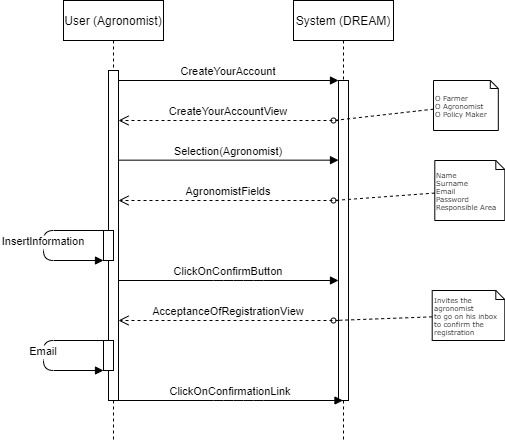
\includegraphics[width=1.0\textwidth]{images/sequenceDiagrams/13. SignUpAgronomist.png}
    \par
    \caption{\label{fig:frog}Sign Up Agronomist}

    \newpage
    
    
    
    
    
    
    
    
    %AGRONOMIST ANSWER TO A REQUEST FOR HELP AND SUGGESTIONS OF FARMERS
    
    \begin{longtable}{|c| p{10cm}|}
        \hline
            ID & 14 \\
        \hline
            Name & Agronomist answers to “Request for Help and Suggestions” of farmers\\
        \hline
            Actor & Agronomist \\
        \hline
            Entry Conditions &  \begin{itemize}
                                    \item Agronomist has logged in
                                    \item Agronomist has received a request for help
                                \end{itemize}\\
        \hline
            Input & Text of the response\\
        \hline
            Events Flow &   \begin{itemize}
                                \item Agronomist clicks on “Requests” 
                                        \begin{itemize}
                                            \item If agronomist directly clicks on the notification of the request, jumps directly to 4th point
                                        \end{itemize}
                                \item System displays a page with a list of the most recent received requests
                                \item Agronomist selects a request
                                \item System displays the request and an “Answer” button
                                \item Agronomist reads the request and selects the “Answer” button
                                \item System displays a text field for the response and a “Send” button
                                \item Agronomist inserts the text and presses the “Send” button
                                \item System shows a message saying “Message sent” 
                                \item System displays agronomist’s home page
                                \item System sends a notification to the sender of the request
                            \end{itemize} \\
        \hline
            Exit Conditions & Response has been sent successfully \\
        \hline
            Output &    \begin{itemize}
                            \item The response is stored in the database of the application
                            \item Sender of the request gets a notification
                        \end{itemize}\\
        \hline
            Exceptions & \begin{itemize}
                            \item Agronomist selects the “Send” button with an empty message for the response. Systems shows an error message “A response can’t be empty” and displays again the page with the text field and the button.
                            \item Agronomist inserts a message in the text field of over 400 characters. Systems shows an error message “A response can have at most 400 characters” and displays again the page with the text field (filled with old message) and the button.
                        \end{itemize}\\
        \hline
    \end{longtable}
    
    \newpage
    
    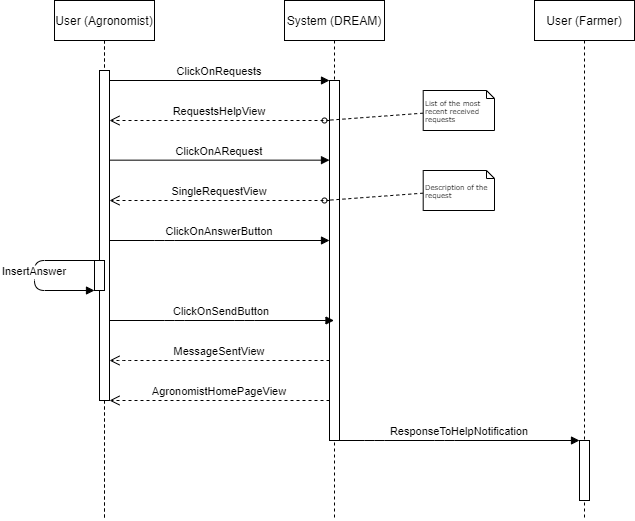
\includegraphics[width=1.0\textwidth]{images/sequenceDiagrams/14. AgronomistRespondHelp.png}
    \par
    \caption{\label{fig:frog}Agronomist answers to “Request for Help and Suggestions” of farmers}

    \newpage
    
    
    
    
    
    
    
    %AGRONOMIST VISUALIZES DAILY PLAN
    
    \begin{longtable}{|c| p{10cm}|}
        \hline
            ID & 15 \\
        \hline
            Name & Agronomist visualizes daily plan\\
        \hline
            Actor & Agronomist \\
        \hline
            Entry Conditions &  \begin{itemize}
                                    \item Agronomist has logged in
                                    \item Agronomist is on his home page
                                    \item Agronomist has already inserted the daily plan he wants to read
                                \end{itemize}\\
        \hline
            Input & \\
        \hline
            Events Flow &   \begin{itemize}
                                \item Agronomist clicks on “Daily Plan” 
                                        \begin{itemize}
                                            \item If agronomist is interested in the daily plan of the following day clicks directly “Read More”, and jumps directly to 4th point
                                        \end{itemize}
                                \item System displays a calendar where a day is coloured if the daily plan of that day has already been inserted
                                \item Agronomist selects one of the coloured days
                                \item System displays the daily plan of the selected day with:
                                        \begin{itemize}
                                            \item If the daily plan is of a future day -> a button “Update” 
                                            \item If the daily plan is of a past day -> the String “Confirmed Daily Plan” or the specified deviations 
                                            \item If the daily plan is of the current day -> the String “Confirmed Daily Plan” or the specified deviations if they’ve already been inserted, otherwise the button “Confirm/Specify Deviations”
                                        \end{itemize}
                            \end{itemize} \\
        \hline
            Exit Conditions & Daily plan is successfully visualized \\
        \hline
            Output & Daily plan is shown to the Agronomist\\
        \hline
            Exceptions & \begin{itemize}
                            \item Agronomist selects a non-coloured day. The system shows the page of the insertion of a daily plan and continues with that use-case.
                            \item Agronomist has no daily plan available (all days are non-coloured). The agronomist can only return to the home page or add a new daily plan.
                        \end{itemize}\\
        \hline
    \end{longtable}
    
    \newpage
    
    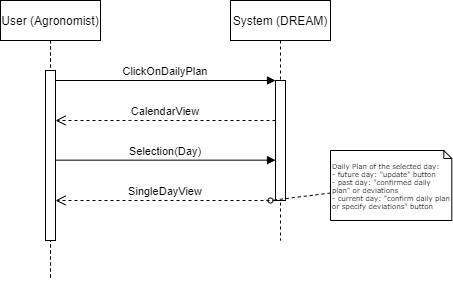
\includegraphics[width=1.0\textwidth]{images/sequenceDiagrams/15. AgronomistVisualizeDailyPlan.png}
    \par
    \caption{\label{fig:frog}Agronomist visualizes daily plan}

    \newpage
    
    
    
    
    
    
    
    
    
    
    %AGRONOMIST UPDATES DAILY PLAN
    
    \begin{longtable}{|c| p{10cm}|}
        \hline
            ID & 16 \\
        \hline
            Name & Agronomist updates a daily plan\\
        \hline
            Actor & Agronomist \\
        \hline
            Entry Conditions &  \begin{itemize}
                                    \item Agronomist has logged in
                                    \item Agronomist is on his home page
                                    \item Agronomist has already inserted the daily plan he wants to update
                                    \item Agronomist is performing the update at least one day before the one of the daily plan
                                \end{itemize}\\
        \hline
            Input & Changes in the daily plan \\
        \hline
            Events Flow &   \begin{itemize}
                                \item Agronomist clicks on “Daily Plan”  
                                        \begin{itemize}
                                            \item If agronomist is interested in the daily plan of the following day clicks directly “Read More”, and jumps directly to 4th point
                                        \end{itemize}
                                \item System displays a calendar where a day is coloured if the daily plan of that day has already been inserted
                                \item Agronomist selects one of the coloured days
                                \item System displays the daily plan of the selected day with:
                                        \begin{itemize}
                                            \item If the daily plan is of a future day -> a button “Update” 
                                            \item If the daily plan is of a past day -> the String “Confirmed Daily Plan” or the specified deviations 
                                            \item If the daily plan is of the current day -> the String “Confirmed Daily Plan” or the specified deviations if they’ve already been inserted, otherwise the button “Confirm/Specify Deviations”
                                        \end{itemize}
                                \item Agronomist clicks on the “Update” button (assuming it’s present)
                                \item System shows a “Save” button and each activity of the daily plan with its own start, end time and description, all in editable fields. 
                                \item Agronomist updates the daily plan modifying the editable fields and clicks on “Save” button
                                \item System shows a message “Daily plan updated successfully” 
                                \item System displays the calendar of the daily plans
                            \end{itemize} \\
        \hline
            Exit Conditions & Daily plan is updated successfully \\
        \hline
            Output & The selected daily plan is updated in the database of the application\\
        \hline
            Exceptions & \begin{itemize}
                            \item Agronomist selects a non-coloured day. The system shows the page of the insertion of a daily plan and continues with that use-case.
                            \item Agronomist has no daily plan available (all days are non-coloured). The agronomist can only return to the home page or add a new daily plan.
                            \item Agronomist tries to modify the daily plan overlapping 2 events. The system shows a message saying “You can’t overlap 2 visits” and displays again the editable daily plan.
                            \item Agronomist tries to modify the daily plan by leaving one of the fields empty. The system shows a message saying “All the fields must be filled” and displays again the editable daily plan.
                            \item Agronomist tries to modify the daily plan of the current day or of a past day. System simply doesn’t display the “Update” button 
                        \end{itemize}\\
        \hline
    \end{longtable}
    
    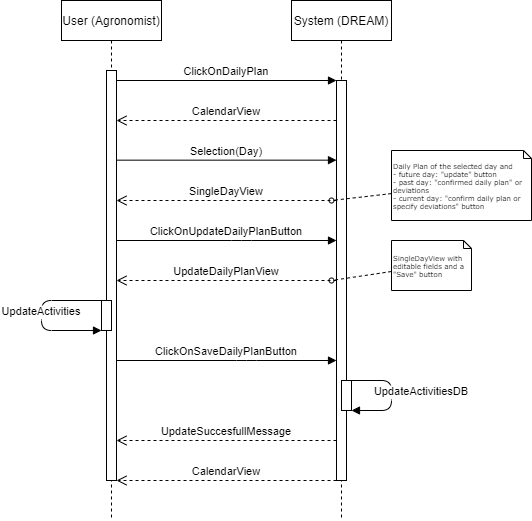
\includegraphics[width=0.9\textwidth]{images/sequenceDiagrams/16. AgronomistUpdateDailyPlan.png}
    \par
    \caption{\label{fig:frog}Agronomist updates daily plan}

    \newpage
    
    
    
    
    
    
    
    
    
    %AGRONOMIST INSERTS DAILY PLAN
    
    \begin{longtable}{|c| p{10cm}|}
        \hline
            ID & 17 \\
        \hline
            Name & Agronomist inserts a daily plan\\
        \hline
            Actor & Agronomist \\
        \hline
            Entry Conditions &  \begin{itemize}
                                    \item Agronomist has logged in
                                    \item Agronomist is on his home page
                                \end{itemize}\\
        \hline
            Input & New daily plan \\
        \hline
            Events Flow &   \begin{itemize}
                                \item Agronomist clicks on “Daily Plan” 
                                \item System displays a calendar where a day is coloured if the daily plan of that day has already been inserted
                                \item Agronomist selects one of the non-coloured days
                                \item System displays
                                            \begin{itemize}
                                                \item 3 editable fields (start, end time and description of the task) for the first activity 
                                                \item The button “Add Activity”
                                                \item The button “Save”
                                            \end{itemize}
                                \item Agronomist compiles the editable fields of the activity 
                                            \begin{itemize}
                                                \item Selects “Save” if all the tasks of his daily plan have been inserted (go ahead to 6th point)
                                                \item Selects “Add Activity” if he wants to add another activity, and the system displays the 3 fields of a new activity and the 2 buttons (back to 3rd point)
                                            \end{itemize}
                                \item System checks if the daily plan is coherent and shows a message “Daily plan inserted successfully”
                                \item System displays the calendar of the daily plans
                            \end{itemize} \\
        \hline
            Exit Conditions & Daily plan is inserted successfully \\
        \hline
            Output & The daily plan is inserted in the database of the application\\
        \hline
            Exceptions & \begin{itemize}
                            \item Agronomist selects a coloured day. The system shows the daily plan as in the visualize/update daily plan use cases.
                            \item Agronomist tries to insert a daily plan overlapping 2 events. The system shows a message saying “You can’t overlap 2 visits” and displays again the editable daily plan.
                            \item Agronomist tries to insert a daily plan with one (or 2) of the fields of an activity empty. The system shows a message saying “All the fields must be filled” and displays again the editable daily plan.
                        \end{itemize}\\
        \hline
    \end{longtable}
    
    \newpage
    
    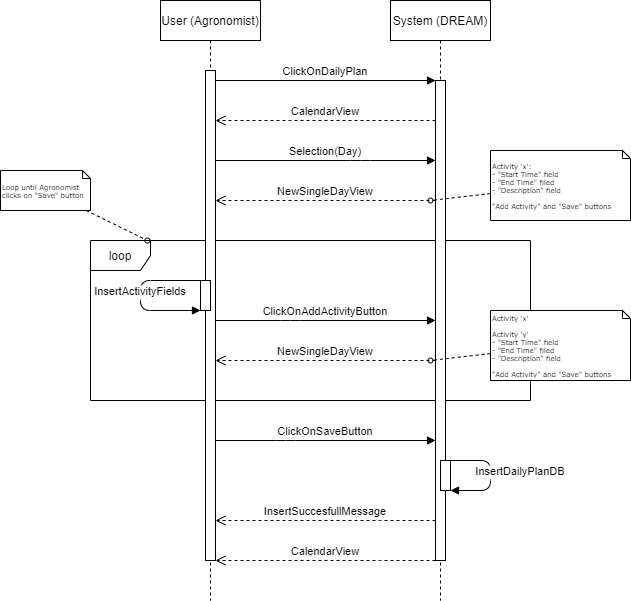
\includegraphics[width=1.0\textwidth]{images/sequenceDiagrams/17. AgronomistInsertDailyPlan.png}
    \par
    \caption{\label{fig:frog}Agronomist inserts daily plan}

    \newpage
    
    
    
    
    
    
    
    
    
    %AGRONOMIST CONFIRMS DAILY PLAN
    
    \begin{longtable}{|c| p{10cm}|}
        \hline
            ID & 18 \\
        \hline
            Name & Agronomist confirms the execution of the daily plan, or specifies deviations\\
        \hline
            Actor & Agronomist \\
        \hline
            Entry Conditions &  \begin{itemize}
                                    \item Agronomist has logged in
                                    \item Agronomist is on his home page
                                \end{itemize}\\
        \hline
            Input & Optional: deviations from the daily plan \\
        \hline
            Events Flow &   \begin{itemize}
                                \item Agronomist clicks on “Daily Plan” 
                                \item System displays a calendar where a day is coloured if the daily plan of that day has already been inserted
                                \item Agronomist selects the current day 
                                \item System displays the daily plan of the selected day with the button “Confirm/Specify Deviations” 
                                \item Agronomist clicks “Confirm/Specify Deviations”
                                \item System displays a page with a field “Add here your deviations from the daily plan” and a button “Confirm”
                                \item Farmer inserts deviations if presents and clicks “Confirm” (if no deviations are specified the daily plan will be considered as without any deviations, so executed perfectly)
                                \item System shows the message “Today’s work successfully confirmed” 
                                \item System displays agronomist’s home page
                            \end{itemize} \\
        \hline
            Exit Conditions & Daily plan is successfully confirmed or deviations are successfully specified \\
        \hline
            Output & The confirmation (and eventual deviations) of the daily plan is inserted in the database of the application\\
        \hline
            Exceptions & \begin{itemize}
                            \item Agronomist still hasn’t inserted a daily plan for the current day. The system continues with the insert daily plan use case, and only after the insertion the user will be able to restart with this use case
                            \item Agronomist selects a day which is not the current one. The system simply won't’ display the button “Confirm/specify deviations” but will display the daily plan of the selected day with:
                                    \begin{itemize}
                                        \item if has selected a future day -> a button “Update”
                                        \item if has selected a past day -> the String “confirmed daily plan” or the specified deviations 
                                    \end{itemize}

                            \item Agronomist tries to confirm/specify deviations to the current day but he has already done it. The system simply displays the daily plan of the selected day with the String “confirmed daily plan” or the specified deviations if they’ve been inserted
                        \end{itemize}\\
        \hline
    \end{longtable}
    
    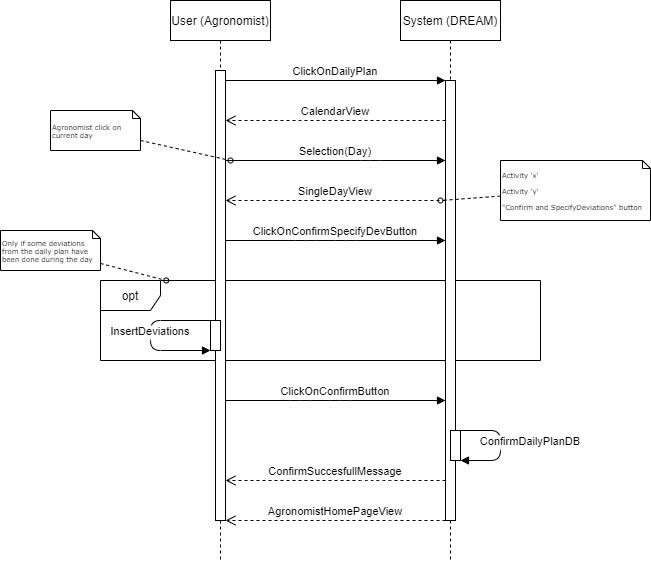
\includegraphics[width=1.0\textwidth]{images/sequenceDiagrams/18. AgronomistConfirmDailyPlan.png}
    \par
    \caption{\label{fig:frog}Agronomist confirms daily plan or specify deviations}

    \newpage
    
    
    
    
    
    
    
    
    
    
    
    
    %AGRONOMIST VISUALIZES PERFORMANCE DATA
    
    \begin{longtable}{|c| p{10cm}|}
        \hline
            ID & 19 \\
        \hline
            Name & Agronomist visualizes performances (production data) of the farmers\\
        \hline
            Actor & Agronomist \\
        \hline
            Entry Conditions &  \begin{itemize}
                                    \item Agronomist has logged in
                                    \item Agronomist is on his home page
                                \end{itemize}\\
        \hline
            Input &  \\
        \hline
            Events Flow &   \begin{itemize}
                                \item Agronomist clicks on “Farmer’s performance” 
                                            \begin{itemize}
                                                \item If agronomist clicks on a received notification of a reported bad performing farmer, in this case jump directly to 4)
                                            \end{itemize}
                                \item System displays:
                                            \begin{itemize}
                                                \item A graph with the result of the current year of his area compared to the same period of the previous one 
                                                \item A list of farmers ordered by performances from the best one to the worst one 
                                                \item A button “Order from worst performances” to reverse the order
                                            \end{itemize}
                                \item Agronomist selects one of the farmers
                                \item System displays the production of the selected farmer
                                            \begin{itemize}
                                                \item Amount of corn produced
                                                \item Amount of energy used per unit
                                                \item Amount of fertilizer used per unit
                                                \item Amount of water used per unit
                                            \end{itemize}
                            \end{itemize} \\
        \hline
            Exit Conditions & Agronomist has successfully checked the production of the selected farmer\\
        \hline
            Output & Agronomist sees farmer’s performances\\
        \hline
            Exceptions & \\
        \hline
    \end{longtable}
    
    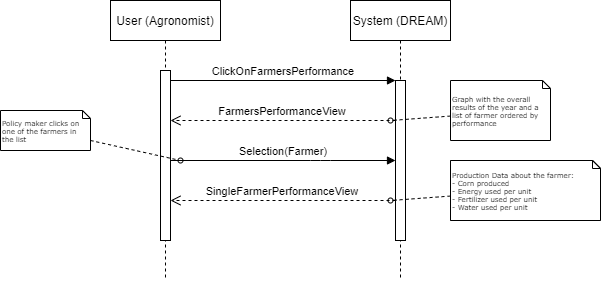
\includegraphics[width=0.8\textwidth]{images/sequenceDiagrams/19. AgronomistVisualizeFarmerPerformance.png}
    \par
    \caption{\label{fig:frog}Agronomist visualizes performances (production data) of the farmers}

    \newpage
    
    
    
\end{center}

    


\subsubsection{Policy Maker use cases}


\begin{center}
    
    
    %POLICY MAKER SIGN UP
    
    \begin{longtable}{|c| p{10cm}|}
        \hline
            ID & 20 \\
        \hline
            Name & Sign Up Agronomist\\
        \hline
            Actor & Policy Maker \\
        \hline
            Entry Conditions & Policy Maker  has downloaded and opened the application on his smartphone (on the “Initial App Screen”), or has opened the web page on his personal computer (on the “Initial Web Page”).\\
        \hline
            Input & \begin{itemize}
                        \item Email to use for the registration
                        \item Personal data (name, surname)
                    \end{itemize}\\
        \hline
            Events Flow &   \begin{itemize}
                                \item Policy maker clicks on “Create your Account”
                                \item System displays a list of alternatives:
                                        \begin{itemize}
                                            \item Farmer
                                            \item Agronomist
                                            \item Policy Maker
                                        \end{itemize}
                                \item Policy Maker selects “Policy Maker”
                                \item System displays a list of fields that the policy maker must compile:
                                        \begin{itemize}
                                            \item Name
                                            \item Surname
                                            \item Email
                                            \item Password
                                        \end{itemize}
                                \item Policy Maker inserts the mandatory data and accepts the Terms of Services
                                \item Policy Maker clicks on “Confirm” button
                                \item System displays the acceptance of registration and invites policy maker to go on his inbox in order to confirm the registration
                                \item Policy Maker opens his inbox, checks the emails and clicks on confirmation link
                            \end{itemize} \\
        \hline
            Exit Conditions & Policy maker registration has been successful: policy maker data is stored in the database of the system. 
                            Policy maker can now login with his credentials (email and password) \\
        \hline
            Output & \begin{itemize}
                        \item The email of the policy maker is stored in the database of the application
                        \item The policy maker receives the email of confirmation
                    \end{itemize}\\
        \hline
            Exceptions & \begin{itemize}
                            \item Policy maker inserts an email which is already stored in the database. So, after the policy maker inserts his data and clicks on confirm, the application displays an error page which tells that policy maker is already registered to the service and invites him to login with that email.
                            \item Policy maker inserts an invalid email. So, after the policy maker clicks on the confirm button, the application displays the same page and an error message, which suggests to the policy maker to check the email inserted or to change it.
                            \item Policy maker inserts invalid data (e.g., the user is not a policy maker), so, after the policy maker clicks on confirm, the application displays an error page which tells that policy maker has inserted invalid data and invites him to try again the registration.
                        \end{itemize}\\
        \hline
    \end{longtable}
    
    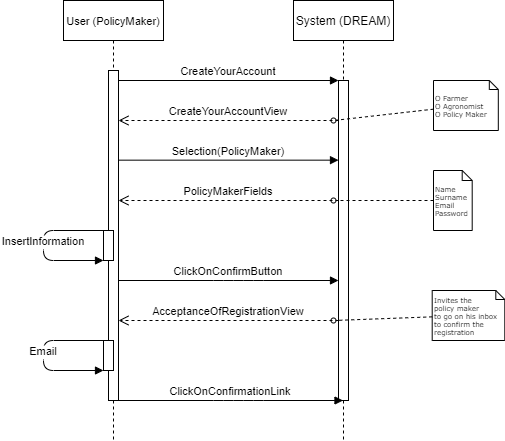
\includegraphics[width=1.0\textwidth]{images/sequenceDiagrams/20. SignUpPolicyMaker.png}
    \par
    \caption{\label{fig:frog}Sign Up Policy Maker}

    \newpage
    
    
    
    
    
    
    
    
    %POLICY MAKER VISUALIZE PERFORMANCES
    
    \begin{longtable}{|c| p{10cm}|}
        \hline
            ID & 21 \\
        \hline
            Name & Policy Maker visualize performances (production data) of the farmers \\
        \hline
            Actor & Policy Maker \\
        \hline
            Entry Conditions &  \begin{itemize}
                                    \item Policy maker has logged in
                                    \item Policy maker is on his home page
                                \end{itemize}\\
        \hline
            Input &  \\
        \hline
            Events Flow &   \begin{itemize}
                                \item Policy maker clicks on “Farmer’s performance” 
                                \item System displays:
                                                \begin{itemize}
                                                    \item A graph with the overall result of the current year compared to the same period of the previous one
                                                    \item A list of farmers ordered by performances from the best one to the worst one 
                                                    \item A button “Order from worst performances” to reverse the order
                                                \end{itemize}

                                \item Policy maker selects one of the farmers
                                \item System displays the production of the selected farmer:
                                                \begin{itemize}
                                                    \item Amount of corn produced
                                                    \item Amount of energy used per unit
                                                    \item Amount of fertilizer used per unit
                                                    \item Amount of water used per unit 
                                                    \item If the farmer is performing better than the average (and hasn’t received a best-practices request in the last 40 days) a button “Ask for best practices”
                                                \end{itemize}
                            \end{itemize} \\
        \hline
            Exit Conditions & Policy maker has successfully checked the overall production and the production of a selected farmer \\
        \hline
            Output & Policy maker sees information about crops and farmers production\\
        \hline
            Exceptions &  \\
        \hline
    \end{longtable}
    
    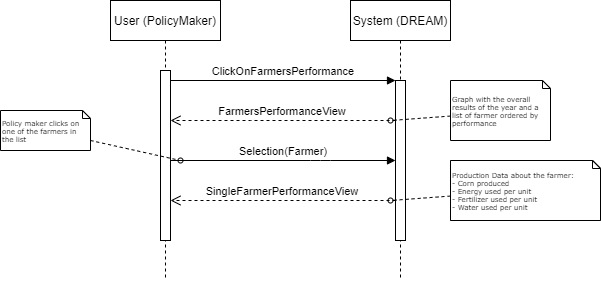
\includegraphics[width=0.8\textwidth]{images/sequenceDiagrams/21. PolicyMakerVisualizeFarmerPerformance.png}
    \par
    \caption{\label{fig:frog}Policy Maker Visualize Performance Data of Farmers}

    \newpage
    
    
    
    
    
    
    %POLICY MAKER ASKS FOR BEST PRACTICES TO A FARMER
    
    \begin{longtable}{|c| p{10cm}|}
        \hline
            ID & 22 \\
        \hline
            Name & Policy Maker asks for “Best Practices” to a farmer \\
        \hline
            Actor & Policy Maker \\
        \hline
            Entry Conditions &  \begin{itemize}
                                    \item Policy maker has logged in
                                    \item Policy maker is on his home page
                                \end{itemize}\\
        \hline
            Input &  \\
        \hline
            Events Flow &   \begin{itemize}
                                \item Policy maker clicks on “Best Practices” 
                                                \begin{itemize}
                                                    \item Policy Maker can also click on “Farmer’s performance”, select a farmer and click on “Ask for best practices” if the button is present; in this case jump directly to 5th point.
                                                \end{itemize}
                                \item System displays a list of the farmers performing better than the average ordered by performances (from the best one) where farmers which have already received a request in the past 40 days are marked.
                                \item Policy maker selects one of the top farmers (the higher it is the best it is performing)
                                \item System displays the production of the selected farmer:
                                                \begin{itemize}
                                                    \item Amount of corn produced
                                                    \item Amount of energy used per unit
                                                    \item Amount of fertilizer used per unit
                                                    \item Amount of water used per unit 
                                                    \item ○	A button “Ask for Best Practices”
                                                \end{itemize}
                                \item System displays a text field pre-compiled saying “You have performed very well recently, can you share some advice?” and a button “Send”
                                \item Policy maker modifies the message if needed and clicks “Send” button
                                \item System notifies the farmer receiver of the request
                                \item System shows the message “Request of best practices successfully sent”
                                \item System displays the “Best Practices” section
                            \end{itemize} \\
        \hline
            Exit Conditions & Policy maker has successfully requested best practices to a well performing farmer \\
        \hline
            Output & Request of best practices is sent to selected the farmer\\
        \hline
            Exceptions & Policy maker selects a marked farmer, trying to ask for best practices to a farmer which has already received a request in the last 40 days. When the policy maker clicks on “Ask for best practices”, the system shows the message “You have already requested best practices to this farmer in the last 40 days” and displays the Best practices section again.\\
        \hline
    \end{longtable}
    
    \newpage
    
    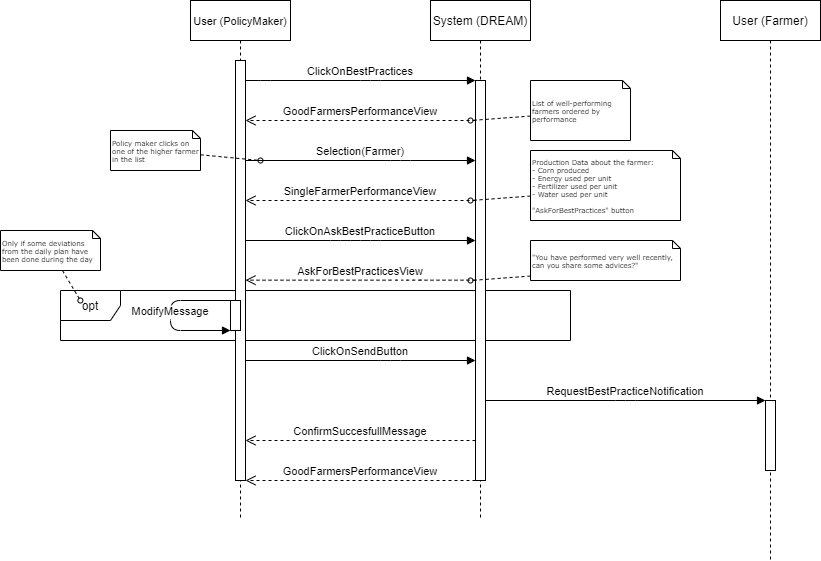
\includegraphics[width=1.0\textwidth]{images/sequenceDiagrams/22. PolicyMakerAskForBestPractice.png}
    \par
    \caption{\label{fig:frog}Policy Maker Ask for Best Practices to well-performing Farmers}

    \newpage
    
    
    
    
    
    
    
    
    
    %POLICY MAKER REPORTS BAD PERFORMING FARMER
    
    \begin{longtable}{|c| p{10cm}|}
        \hline
            ID & 23 \\
        \hline
            Name & Policy maker reports a bad performing farmer \\
        \hline
            Actor & Policy Maker \\
        \hline
            Entry Conditions &  \begin{itemize}
                                    \item Policy maker has logged in
                                    \item Policy maker is on his home page
                                \end{itemize}\\
        \hline
            Input &  \\
        \hline
            Events Flow &   \begin{itemize}
                                \item Policy maker clicks on “Farmer’s performance”
                                \item System displays
                                            \begin{itemize}
                                                \item A graph with the overall result of the current year compared to the same period of the previous one
                                                \item A list of farmers ordered by performances from the best one to the worst one 
                                                \item A button “Order from worst performances” to reverse the order
                                            \end{itemize}
                                \item Policy maker clicks the button “Order from worst performances”
                                \item System displays again the same page but with farmers ordered in the opposite direction (worst on top) and this time the button “Order from good performances” 
                                \item Policy maker selects a bad performing farmer
                                \item System displays the production of the selected farmer
                                            \begin{itemize}
                                                \item Amount of corn produced
                                                \item Amount of energy used per unit
                                                \item Amount of fertilizer used per unit
                                                \item Amount of water used per unit 
                                                \item If the farmer is performing worse than the average a button “Report as bad Performing”
                                            \end{itemize}
                                \item Policy maker clicks “Report as bad performing”
                                \item System shows the agronomists responsible for the area to which the farmer is related (could be more than 1) and a button “Report”
                                \item Policy maker selects an agronomist and clicks “Report”
                                \item System notifies the selected agronomist with the received report
                                \item System shows the message “Report successfully sent” 
                                \item System displays “Farmer’s performances” section 
                            \end{itemize} \\
        \hline
            Exit Conditions & Policy maker has successfully reported the bad performing farmer \\
        \hline
            Output & Selected agronomist receives the report with the bad performing farmer\\
        \hline
            Exceptions & Policy maker clicks “Report as bad performing” on a farmer already reported  in the last 40 days. The system shows the message “You have already reported this farmer in the last 40 days” and displays the “Farmer’s performances” section again.\\
        \hline
    \end{longtable}
    
    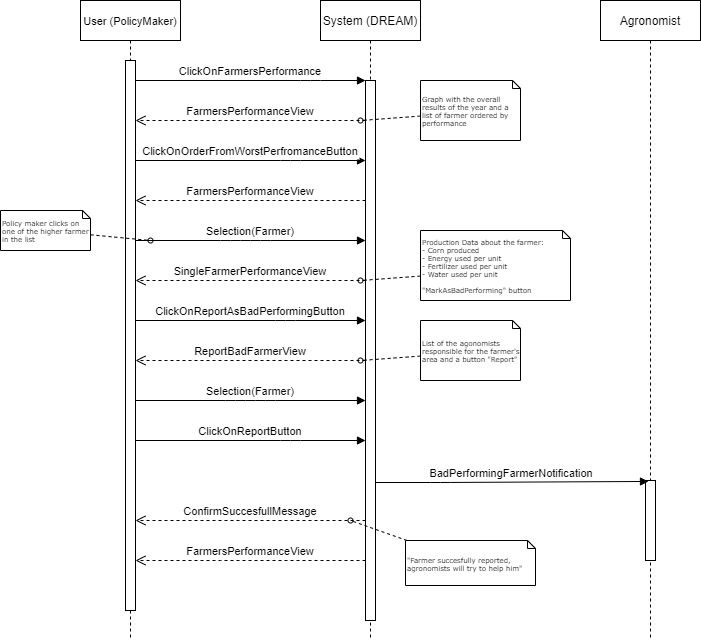
\includegraphics[width=1.0\textwidth]{images/sequenceDiagrams/23. PolicyMakerReportBadFarmers.png}
    \par
    \caption{\label{fig:frog}Policy Maker reports a bad-performing Farmer}

    \newpage
    
    

    
\end{center}




\subsubsection{User use cases}

User stands for general actor, so it could be agronomist, farmer or policy maker.

\begin{center}
    
    %POLICY MAKER REPORTS BAD PERFORMING FARMER
    
    \begin{longtable}{|c| p{10cm}|}
        \hline
            ID & 24 \\
        \hline
            Name & Login user \\
        \hline
            Actor & User (agronomist, farmer, or policy maker) \\
        \hline
            Entry Conditions &  \begin{itemize}
                                    \item User has downloaded and opened the application on his smartphone (on the “Initial App Screen”), or has opened the web page on his personal computer (on the “Initial Web Page”).
                                    \item User has registered to the service
                                \end{itemize}\\
        \hline
            Input &     \begin{itemize}
                            \item Email
                            \item Password
                        \end{itemize}Email \\
        \hline
            Events Flow &   \begin{itemize}
                                \item User inserts “Email” and “Password” in apposite fields
                                \item User clicks on “Login”
                                \item System checks the correctness of the credential inserted
                                \item System displays user’s home page
                            \end{itemize} \\
        \hline
            Exit Conditions & User is logged in \\
        \hline
            Output & System shows user’s home page\\
        \hline
            Exceptions & User inserts wrong credentials. The system displays the login page with an error saying “Wrong credentials”.\\
        \hline
    \end{longtable}
    
    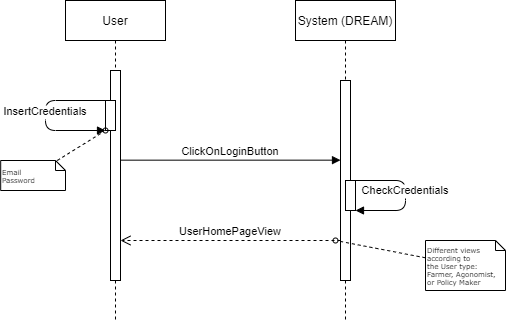
\includegraphics[width=0.9\textwidth]{images/sequenceDiagrams/24. UserLogin.png}
    \par
    \caption{\label{fig:frog}User Login}

    \newpage
    
\end{center}


\subsubsection{Requirements}

    \begin{itemize}
        \item R1: The system shall allow the registration of new users of three different types: farmer, agronomists and policy makers.
        \item R2: The system shall elaborate a list of suggestions for the registered farmer user.
        \item R3: The system shall allow the farmer user to send help or suggestions requests to a selected agronomist user or farmer user.
        \item R4: The system shall send a notification to the farmer user when he receives requests for best practices or new answers or requests in the help requests or forum threads.
        \item R5: The system shall allow a farmer user to read and respond to threads in the farmer forums.
        \item R6: The system shall allow a farmer to insert production data.
        \item R7: The system shall allow the farmer user to respond to a request for best practices.
        \item R8: The system shall present an accurate weather forecast for the days following the current one to both farmer users and agronomists.
        \item R9: The systems shall allow an agronomist user to respond to help and suggestions requests received by farmer users.
        \item R10: The system shall send a notification to the agronomist user when a help request is received or a farmer is reported as “bad performing”.
        \item R11: The system shall present to agronomist users and policy maker users all the performance data that are available.
        \item R12: The system shall allow agronomist users to insert and modify a daily plan
        \item R13: The system shall allow the agronomist to confirm the execution of the daily plan or specify its deviations
        \item R14: The system shall not allow the creation of a daily plan if a farmer is not receiving it’s mandatory visits, that must be at least twice a year, and the day is the last available. Consequently it shall notify the exception to the agronomist user.
        \item R15: The system shall present the daily plan to the agronomist user.
        \item R16: The system shall allow policy maker users to send to farmer users requests for best practices.
        \itemR17: The system shall allow policy maker to report bad performing farmers to agronomists

    \end{itemize}

\newpage

This paragraph will summarize the goals described in section 1.2, showing the requirements and the domain assumptions for each of them.

    \begin{itemize}
        \item G1: Increase the overall welfare and production of the Telangana region.
                        \begin{itemize}
                            \item R2 - R3 - R5 - R6 - R7 - R8 - R9 - R11 - R17
                            \item D1: Users (farmers, agronomists, and policy makers) do not insert false information in the system.
                            \item D2: Farmers reply as best as they can, giving the best advice, to requests for help and suggestions by other farmers.
                            \item D6: Users have access to a stable Internet connection.
                        \end{itemize}
        \item G2: Aid policy makers in the decisional process.
                        \begin{itemize}
                            \item R1 - R6 - R11 - R16 - R17
                            \item D1: Users (farmers, agronomists, and policy makers) do not insert false information in the system.
                            \item D6: Users have access to a stable Internet connection.
                        \end{itemize}                
        \item G3: Aid the farmers in the management of their productions.
                        \begin{itemize}
                            \item R1 - R2 - R3 - R4 - R5 - R6 - R7 - R8 - R9
                            \item D1: Users (farmers, agronomists, and policy makers) do not insert false information in the system.
                            \item D2: Farmers reply as best as they can, giving the best advice, to requests for help and suggestions by other farmers.
                            \item D4: Each area has at least one responsible agronomist.
                            \item D5: Each farm is assigned to a specific area and has a unique identifier. 
                            \item D6: Users have access to a stable Internet connection.
                            \item D7: The location of a farm is known by the application, and the responsible agronomist is able to reach the farm.
                        \end{itemize} 
        \item G4: Aid agronomist works to help farmers and check crops production.
                        \begin{itemize}
                            \item R1 - R3 - R6 - R8 - R9 - R10 - R11 - R12 - R13 - R14 - R15 - R17
                            \item D1: Users (farmers, agronomists, and policy makers) do not insert false information in the system.
                            \item D3: Agronomists know the area they are responsible for.
                            \item D4: Each area has at least one responsible agronomist.
                            \item D6: Users have access to a stable Internet connection.
                            \item D7: The location of a farm is known by the application, and the responsible agronomist is able to reach the farm.
                        \end{itemize} 	
    \end{itemize}



\newpage



\subsection{Software System Attributes}

\subsubsection{Reliability}
The system should be able to run continuously (with maintenance interruption scheduled in less crowded hours) in order to keep all the functionalities accessible with no interruptions (such as the forum). The highest number of simultaneous users is expected at the end of each day when all the agronomists confirm (or specify deviations) their daily plan and farmers control weather forecasts of the following day.

\subsubsection{Availability}
The system must have a minimum availability of 96%.

\subsubsection{Security}
All the information (such as registration data) must be kept private to all non authenticated and authorized users (ex. The location of each farm must be known only to the agronomists related to that area). 
Communication between parties should take place on secure channels in order to provide encryption, authentication and integrity (to prevent interception, modification and fabrication of messages).

\subsubsection{Maintainability}
The code will be well-documented using JavaDoc to enable developers to easily understand it. It will be designed in order to permit future additions of functionalities with minimum effort and will follow the object oriented model-controller-view pattern (to achieve a higher separation of concerns).

\subsubsection{Portability}
The back-end server software will be written in Java and will be able to run on every
platform that supports the JVM. The front end will be supported by the current versions of Safari, Mozilla Firefox and Chrome, and by the latest 3 versions of Android/IOS for the mobile application.




\newpage





\section{Formal analysis using Alloy} 

\subsection{Alloy Code}

\begin{lstlisting}[language=alloy] 

sig Text{}

abstract sig User {
	email: one Email,
	password: one Text,
	name: one Text,
	surname: one Text
}

sig Email{}

sig Farmer extends User {
	farm: one Farm
}

sig Farm {
	farmName: one Text,
	farmPosition: one Position,
	belongingArea: one Area,
	ownerName: one Farmer
}

sig Position{}

sig Agronomist extends User {
	area: one Area,
	plan: one Plan
}

sig Area{}

sig PolicyMaker extends User {}

sig Plan {
	visits: some Visit
}

sig Visit {
	day: one Day,
	initialHour: one Hour,
	endHour: one Hour,
	motivation: one Text,
	farm: one Farm
}

sig Day{}
sig Hour{}

sig ProductionData {
	data: set FarmerProduction
}

sig FarmerProduction {
	cropType: one CropType,
	weather: one WeatherForecast,
	cropQuantity: one CropQ,
	energy: one EnergyQ,
	fertilizer: one Fertilizer,
	water: one WaterQ,
	farm: one Farm,
	day: one Day
}

sig CropType{}
sig CropQ{}
sig EnergyQ{}
sig Fertilizer{}
sig WaterQ{}

sig BestPractices {
	bestPractice: set BestPractice
}

sig BestPractice {
	content: one Text,
	farmerData: one FarmerProduction,
	request: one BestPracticeRequest
}

sig BestPracticeRequest {
	recipientEmail: one Email,
	day: one Day,
	hour: one Hour
}

sig WeatherForecast {
	forecasts: some Forecast
}

sig Forecast {
	day: one Day,
	time: one Hour,
	position: one Position,
	weather: one Weather, //rain, sun, ...
	temperature: one TemperatureQ,
	humidity: one HumidityQ,
	wind: one WindQ
}

sig Weather{}
sig TemperatureQ{}
sig HumidityQ{}
sig WindQ{}

sig HelpAndSuggestions {
	list: set Conversation
}

sig Conversation{
	content: some Message,
	participantUsers: some Email
}

sig Message {
	text: one Text,
	email: one Email,
	day: one Day,
	time: one Hour
}

sig Forum {
	pages: set ForumPage
}

sig ForumPage {
	category: one Text,
	name: one Text,
	posts: set ForumThread
}

sig ForumThread {
	postTitle: one Text,
	creatorFarmer: one Farmer,
	object: one Text,
	messages: set Message
}

sig PersonalizedSuggestions {
	suggestions: set Suggestions,
	destinationFarmer: one Farmer
} 

sig Suggestions{}


--------------------------------------------------------------------



fact {
	//Two user can't have the same email address
	no disj u1, u2: User | u1.email = u2.email
}

fact {
	//Every Area has at least one responsible agronomist
	all a: Area | 
		some b : Agronomist | b.area = a
}

fact {
	//Every farmer is associated to one and only one farm
	all f: Farmer, f2: Farm |
			(f.farm = f2 implies f2.ownerName = f) and 
			(f2.ownerName = f implies f.farm = f2)
}

fact {
	//Two farm can't be in the same position
	no disj f1, f2: Farm | f1.farmPosition = f2.farmPosition
}

fact {
	//Every farmer has a unique personalized suggestion
	all f: Farmer |
		one sug: PersonalizedSuggestions | sug.destinationFarmer = f
}

fact {
	//Every agronomist has a unique plan
	all p : Plan |
		one a : Agronomist | a.plan = p
}

fact {
	//Every mail in a message should belong to a user
	all e: Message.email |
		some u : User | u.email = e
}

fact {
	//Every mail in a conversation should belong to a user
	all e: Conversation.participantUsers |
		some u : User | u.email = e
}

fact {
	//Can't have different forecast for the same time and day
	no disj f1, f2: Forecast |
		f1.day = f2.day and f1.time = f2.time and f1.position = f2.position and
		(f1.temperature != f2.temperature or f1.weather != f2.weather or f1.humidity != f2.humidity or f1.wind != f2.wind)

}

fact { 
	//Message in a conversation must have email only from user participating to the conversation
	all conv: Conversation |
		all mess: conv.content | some participant: conv.participantUsers | mess.email = participant
}

fact {
	//All forum thread must participate to one Forum page
	all ft : ForumThread |
		one fp : ForumPage | ft in fp.posts 
}

fact {
	//The email of the Best practice request must belong to a farmer
	all bpr: BestPracticeRequest |
		one farmer: Farmer | farmer.email = bpr.recipientEmail
}

fact {
	//You can't have a Conversation with a policy maker
	no convEm: Conversation.participantUsers |
		some pm: PolicyMaker | pm.email = convEm
}

fact {
	//All conversation must participate to HelpAndSuggestions
	all c: Conversation |
		c in HelpAndSuggestions.list

}

fact {
	//All Visit must participate to a Plan
	all v: Visit |
		v in Plan.visits

}

fact {
	//A BestPracticeRequest must have mail corresponding to the BestPractice
	all bp: BestPractice |
		bp.request.recipientEmail = bp.farmerData.farm.ownerName.email
}

fact {
	//only farmers can participate to the forum
	all forumEm: ForumThread.messages.email |
		some f: Farmer | f.email = forumEm
}

fact {
	//every visits should belong to the area of competence of the agronomist
	all a: Agronomist |
		all visit: a.plan.visits | a.area = visit.farm.belongingArea
}

fact {
	//all FarmerProduction should belong to ProductionData
	all fp: FarmerProduction |
		one pd: ProductionData | fp in pd.data
}


--------------------------------------------------------------------


//Every farmer has at least one connected agronomist
assert farmerHasAgronomist {
	all f: Farmer | 
		some a: Agronomist | a.area = f.farm.belongingArea
}
//check farmerHasAgronomist

//Every message in conversation must belong to a farmer or an agronomist
assert noPolicyMakerInConversation {
	all c: Conversation |
		all userEm : c.participantUsers | 
			(some f: Farmer | f.email = userEm) or (some a: Agronomist | a.email = userEm)
}
//check noPolicyMakerInConversation

//No message in a conversation has an email different from the participant to the conversation
assert noMessageFromStranger {
	no conv: Conversation |
		some message: conv.content |  
			message.email not in conv.participantUsers
}
//check noMessageFromStranger


--------------------------------------------------------------------


//The first world has the aim to present all communication method present to the farmer
pred world1 {
	#Farmer = 2
	#Agronomist = 1
	#Visit = 2
	#PolicyMaker = 0
	#HelpAndSuggestions = 1
	#Conversation = 2
	#BestPracticeRequest = 0
	#BestPractice = 0
	#ForumThread = 1
	#ForumPage = 2
	#Suggestions = 1
	#Forecast = 0
	#ProductionData = 0
	#WeatherForecast = 0
	#Message = 3
}

//The second world puts the emphasis on the Agronomist and his instruments
pred world2 {
	#Farmer = 2
	#Agronomist = 3
	#Visit = 4
	#PolicyMaker = 0
	#HelpAndSuggestions = 0
	#Conversation = 0
	#BestPracticeRequest = 0
	#BestPractice = 0
	#ForumThread = 0
	#Suggestions = 0
	#Forecast = 0
	#ProductionData = 0
	#WeatherForecast = 0
	#Message = 0
	#Area = 2
	#Forum = 0
	#ForumPage = 0
}

//The third world show what is inherent with the policy maker
pred world3 {
	#Farmer = 2
	#Agronomist = 1
	#Visit = 1
	#PolicyMaker = 2
	#HelpAndSuggestions = 0
	#Conversation = 0
	#BestPracticeRequest = 2
	#BestPractice = 2
	#ForumThread = 0
	#Suggestions = 0
	#Forecast = 1
	#ProductionData = 1
	#FarmerProduction = 2
	#WeatherForecast = 1
	#Message = 0
	#Area = 1
	#Forum = 0
	#ForumPage = 0
	no disj bpr1, bpr2 : BestPracticeRequest | bpr1.recipientEmail = bpr2.recipientEmail
}

//run world1 for 5
//run world2 for 5
//run world3 for 5

\end{lstlisting}

\newpage

\subsection{Worlds}

\subsubsection{World 1}

This world is built to show all the entities that are of most interest to the farmer, to showcase all the possible means of communication he has.

    \begin{figure} [h]
        \centering
        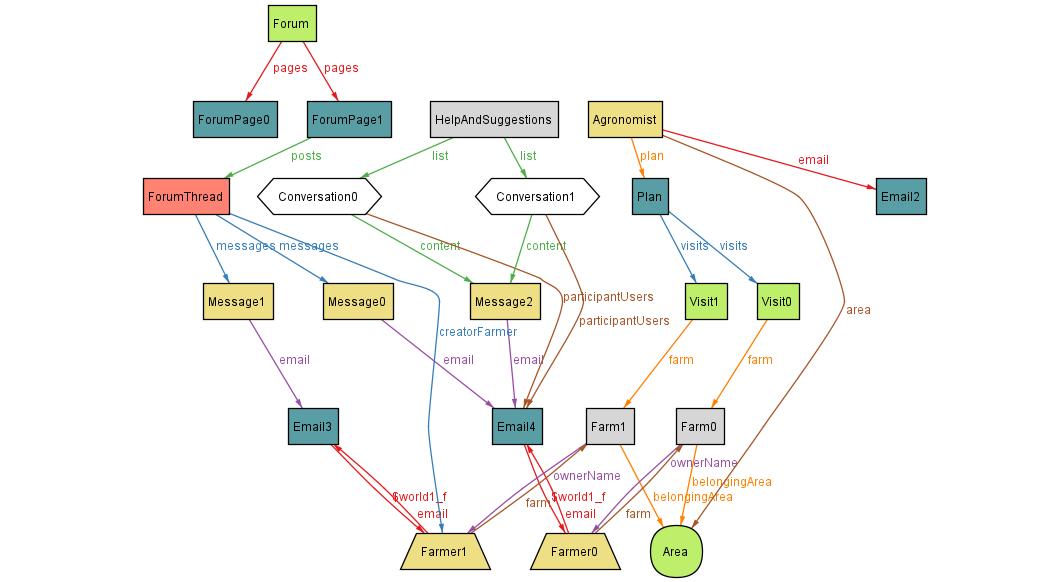
\includegraphics[width=0.9\textwidth]{images/alloy/World1.png}
        \caption{\label{fig:frog}World 1.}
    \end{figure}

\subsubsection{World 2}

This world is built to showcase the plan functionality for the agronomist.

    \begin{figure} [h]
        \centering
        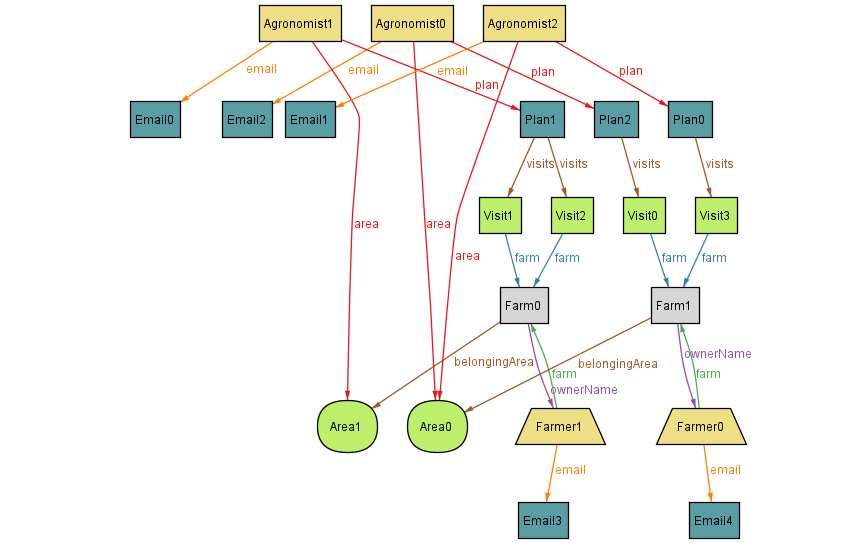
\includegraphics[width=0.8\textwidth]{images/alloy/World2.png}
        \caption{\label{fig:frog}World 2.}
    \end{figure}

\subsubsection{World 3}

This world is built to present to the Policy maker the instruments that he could use to aid his work.

    \begin{figure} [h]
        \centering
        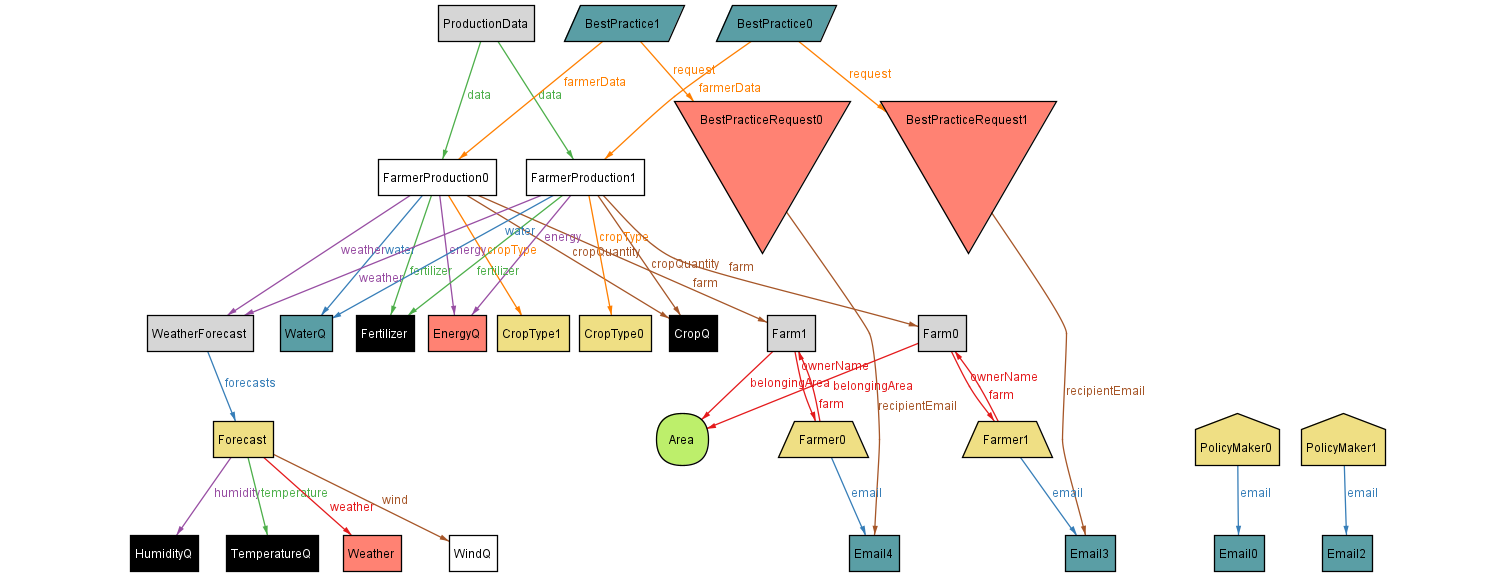
\includegraphics[width=0.9\textwidth]{images/alloy/World3.png}
        \caption{\label{fig:frog}World 3.}
    \end{figure}

\newpage




\section{Effort Spent}


    \begin{longtable}{|p{3cm}|p{2cm}|p{2cm}|p{2cm}|p{2cm}|p{2cm}|}
        \hline
                        & Cap1      & Cap2  & Cap3      & Cap4  & Latex \\
        \hline
            Brunati     & 4h        & 3h    & 14h30min  & 4h    &       \\
        \hline
            Cappelletti & 2h30min   & 5h    & 7h30min   & 4h    & 10h   \\
        \hline 
            Curti       & 4h        & 3h    & 5h        & 11h   &       \\
        \hline    
    \end{longtable}


\end{document}